% !TeX root = bsp.tex

% class options:
% - select either [german] or [english]
% - select the type of thesis from:
%   [bachelor, master, generic]
%   (in case of generic, use \type{} to specify it)
% - use option "alpha" for abbreviated citation (instead of numbers)
% - option "draft" is available, too
% - use options "utf8" or "latin1" to select inputencoding
\documentclass[english, bachelor, utf8]{base/thesis_telematics}

\usepackage{units}    % useful for settings units:              \unit[23]{m}
\usepackage{nicefrac} % for setting fractions esp. within text: \nicefrac{km}{h}
\usepackage{subcaption} % for subfigure environment
\usepackage[utf8]{inputenc}
\usepackage{array} % für bessere Tabellen
\usepackage{geometry}
\geometry{margin=2.5cm}

\usepackage{algorithm, algorithmic}  % for pseudo code (cf. documentation)
\renewcommand{\algorithmiccomment}[1]{\qquad{\small // \textit{#1}}}
\usepackage{tikz}
\usetikzlibrary{arrows.meta, positioning, shapes.geometric, calc}
\usepackage{pdfpages}
\usepackage{hyperref}
\usepackage{booktabs}
\usepackage[utf8]{inputenc}
\usepackage{svg}
\usepackage{subcaption}

%%%%%%%%%%%%%%%%%%%%%%%%%%%%%%%%%%%%%%%%%%%%%%%%%%%%%%%%%%%%%%%%%%%%%%%%%%%%%%%

\begin{document}

\title{Raspberry PI based Camera--LiDAR rig for colored 3D Pointclouds}
\author{Jakob Wehr}
\email{jakob.wehr@stud-mail.uni-wuerzburg.de}
\firstSupervisor{Prof. Dr. Andreas Nuechter}
\secondSupervisor{Dr. Michael Bleier}
\thirdSupervisor{}
%\thirdSupervisor{} %for to give credit to the person supervising but not reviewing the thesis 
%\dept{...}                             % by default Robotics and Telematics
%\submitdate{November 2004}             % by default current month & year
%\signcity{}                            % by default W�rzburg
%signline{W�rzburg, 1. April 2014} % by default "signcity, submitdate"

\generatetitle

\cleardoublepage

\begin{prefacesection}{Abstract}
This Bachelor's thesis presents the design and implementation of a low-cost, handheld \\RGB-D scanning device
built from widely available components -- a Raspberry Pi 5, Raspberry Pi Global shutter camera and a Livox Mid-70
LiDAR -- aimed at producing research-grade datasets for sensor-fusion experiments and Uni-Fusion pipelines
at the same research chair where this work is conducted. The system employs ROS-based recording and a
structured export that tightly couples LiDAR scans and images while ensuring cross-sensor
time synchronization via the Precision Time Protocol (PTP). The processing pipeline generates depth images
and synchronized RGB-D frames for Uni-Fusion, and provides colorized point clouds to inspect extrinsic
calibration. With a bill of materials of $\sim$EUR 1{,}500, the prototype demonstrates a genuinely low-cost
platform suitable for teaching labs and exploratory research. Experiments confirm end-to-end functionality
but also reveal remaining limitations -- most notably imperfect LiDAR-camera extrinsic calibration and an
as-yet uncalibrated external IMU -- while full Uni-Fusion evaluation remains prepared but untested due to
target-system constraints.
\end{prefacesection}

\cleardoublepage
\tableofcontents


\startTextChapters %%%%%%%%%%%%%%%%%%%%%%%%%%%%%%

\chapter{Introduction}

The rapid progress in three-dimensional (3D) sensing technologies has significantly expanded the possibilities 
for spatial data acquisition in diverse domains such as robotics, autonomous navigation, cultural heritage 
documentation and construction monitoring. A key advancement in this context has been the emergence of 
RGB-D imaging, which captures both the color (RGB) and depth (D) information of a scene in a single system. 
By combining semantic richness from visual data with the geometric accuracy of depth measurements, RGB-D 
approaches enable detailed and meaningful 3D reconstructions that are crucial for a wide range of applications.

The popularization of low-cost RGB-D devices, most prominently the Microsoft Kinect, represents a milestone 
in this development. The first generation Kinect employed a PrimeSense structured-light depth sensor, which 
allowed real-time depth estimation but was limited in outdoor environments due to sensitivity to sunlight. 
Later iterations, such as the Kinect v2 and Azure Kinect, shifted to time-of-flight (ToF) sensors, extending 
the maximum measurable range up to approximately 7.5 meters~\cite{3dpclecture}. While this marked a considerable 
improvement over structured-light solutions, the technology continued to face limitations in terms of range, 
accuracy and robustness, particularly in uncontrolled outdoor conditions where strong ambient illumination 
interferes with infrared-based measurements.

To overcome such restrictions, several alternatives have been explored in recent years. One approach relies 
on the use of multiple cameras to generate dense reconstructions through photogrammetric methods. By leveraging 
multi-view geometry and at least one RGB sensor for color encoding, photogrammetry can provide accurate depth 
over larger distances, but at the expense of high computational requirements and sensitivity to textureless 
surfaces. Another method combines RGB cameras with structured infrared patterns and inertial measurement units, 
as seen in devices such as the Intel RealSense D455. Although effective in indoor environments, these systems 
remain vulnerable to degradation in bright outdoor light. A third and increasingly promising avenue is the 
integration of RGB cameras with LiDAR sensors. LiDAR, by actively emitting laser pulses and measuring their 
returns, offers high robustness to illumination conditions and can capture accurate depth across larger ranges. 
The falling costs of compact LiDAR units have further strengthened their appeal for mobile and handheld 
applications.

The objective of this thesis is to design and implement a handheld device that employs an RGB camera in 
combination with a low-cost Livox LiDAR scanner to achieve reliable outdoor depth sensing. This system aims 
to circumvent the weaknesses of structured-light or infrared-based methods under sunlight, while leveraging 
the complementary strengths of LiDAR and RGB imaging. The handheld design not only emphasizes portability 
and ease of use, but also opens opportunities for rapid on-site 3D data acquisition without the constraints 
of bulky equipment.

Recent research has demonstrated the potential of combining LiDAR with vision sensors for dense depth map 
generation in outdoor environments. A notable contribution in this area is the work by Bleier, Yuan and 
Nüchter~\cite{bleier2024}, who introduced a handheld stereo vision and LiDAR system capable of producing dense 
RGB-D maps by applying depth map completion based on learned priors. Their system exploits stereo cameras to 
capture visual data and a low-cost automotive LiDAR to supply sparse but metrically accurate depth information. 
By applying deep learning techniques to complete the sparse LiDAR data, they were able to generate dense depth 
maps with both accuracy and efficiency, even in challenging outdoor settings. This work provides an important 
methodological reference and demonstrates that the combination of vision and LiDAR, supported by learned priors, 
can significantly enhance the quality of handheld 3D mapping systems.

Further contributions in the literature similarly explore handheld systems that fuse monocular 
vision with LiDAR, each addressing specific challenges.

One influential study by Behari et al. at CVPR 2025~\cite{behari2025blurred} introduces a handheld setup that 
combines RGB imaging with a diffuse (blurred) LiDAR sensor. While conventional sparse 
LiDARs often fail to cover the entire scene, the diffuse LiDAR emits a wide-field flash, improving 
coverage but producing ambiguous multi-return signals. To address this, the authors propose a 
Gaussian surfel-based rendering framework together with a scene-adaptive loss, 
which balances the geometric accuracy of LiDAR with the semantic richness of RGB cues. This method 
enables robust handheld 3D scanning even in challenging environments with low texture, low albedo
or limited lighting, thereby outperforming traditional sparse LiDAR approaches.

Another notable contribution is presented by Lin et al.~\cite{lin2024lidarmirror}, who focused on 
mapping specular and transparent surfaces using a consumer-grade flash LiDAR integrated 
into a handheld smartphone device. Standard LiDAR systems typically assume single-bounce 
reflections, which leads to missing data when scanning mirrors or glass. To overcome this, the 
authors introduced a reciprocal pair algorithm that explicitly detects and reconstructs 
multi-bounce returns. Their approach enables accurate, real-time handheld reconstructions of 
reflective and transparent objects, extending the applicability of low-cost LiDAR sensors.

In addition to novel sensing concepts, the Newer College Dataset by Ramezani et al.
~\cite{ramezani2019newer} provides a valuable benchmark for handheld mapping. The dataset was 
recorded with a handheld device combining a stereo-inertial camera and a multi-beam 3D LiDAR while 
walking through a university campus. By aligning this data with a survey-grade reference map, the 
authors provide centimeter-accurate 6-DoF ground truth. This resource is essential for evaluating 
the performance of handheld LiDAR--vision fusion systems and highlights the practical challenges of 
sensor alignment and outdoor robustness.

These studies emphasize three central aspects: addressing sparse LiDAR coverage through novel sensor 
designs (Behari et al.), handling challenging material properties such as reflections and 
transparency (Lin et al.) and enabling reproducible evaluation through high-quality handheld 
datasets (Ramezani et al.). Together, they strengthen the evidence for the relevance of combining 
LiDAR and monocular vision in mobile or handheld 3D reconstruction systems.

Against this backdrop, the present thesis contributes to the field by developing a prototype low-cost handheld device 
that integrates a Livox LiDAR scanner with an RGB camera. The design encompasses both the hardware construction 
and the software implementation required for sensor synchronization, calibration and generating RGB-D frames
as input to the Uni-Fusion framework proposed by Yuan et al.~\cite{yuan2024uni}.

\section*{Task definition}
This thesis focuses on the design and implementation of a low-cost, handheld RGB-D scanning device using
widely available components, specifically a Raspberry Pi~5 (16GB) as the processing platform, a Raspberry Pi camera
module for RGB image capture and a Livox Mid-70 LiDAR scanner for depth acquisition. The primary goal is to
develop a portable system capable of producing RGB-D datasets suitable for sensor fusion experiments -- particularly Uni--Fusion -- without relying on expensive commercial solutions.

The research addresses the complete pipeline: from hardware integration and calibration of the monocular
camera--LiDAR system, through data acquisition, to post-processing and alignment of RGB
and depth streams. Special attention is given to cost-efficiency, portability, and the reproducibility of the system
design, so that it can be easily replicated and is also affordable for amateurs.

In summary, the aim of this work is to:
\begin{itemize}
    \item Design and build a handheld, low-cost RGB-D device using a Raspberry Pi~5, monocular camera and
    Livox Mid-70 LiDAR scanner.
    \item Implement a calibration and synchronization method for accurate data acquisition.
    \item Designing a system that can process the recorded data and create dense depth images.
    \item Creating output that can be processed by Uni-Fusion.
    \item Demonstrate that the system fulfills its purpose and that Uni-Fusion can process the generated RGB-D files.
\end{itemize}

By achieving these objectives, this work should make it easier for tech enthusiasts to get started with handheld devices, LiDAR scanners
and processing RBG-D data, thanks to the low price of the complete system.

\chapter{State of the Art}

\section*{Handheld stereo vision and LiDAR system (University Wuerzburg Computer Science XVII)}
Bleier et al.~\cite{bleier2024} present a custom-built handheld mapping system designed to 
capture dense RGB-D data in outdoor environments using low-cost sensors. The hardware integrates 
a stereo camera pair and a low-cost automotive LiDAR (specifically, a Livox Avia sensor) mounted on a 
commercial camera rig (e.g., NEEWER CA016 Cage, Figure~\ref{fig:bleier_handheld_design}). The system 
also houses embedded electronics including a single-board computer, power management, cooling 
elements, and features a handle and Wi-Fi antenna for operation and data transfer.

The core innovation resides in combining sparse LiDAR measurements with monocular RGB-based depth 
estimation to generate dense, metrically accurate RGB-D frames with low latency. To that end, they 
employ a modern monocular depth estimator (Metric3Dv2, Hu et al., 2024) and subsequently apply learned 
scale correction using sparse LiDAR returns as ground truth priors. This enables the generation of 
dense depth maps from just one sparse scan and a single image, circumventing the need for multi-view 
bundle adjustment or LiDAR scan aggregation.

For validation, the authors compare the learning-based depth completion to traditional LiDAR-only 
mapping via scan matching. While the baseline model-based regression performs worse in their experiments, 
it still achieves dense RGB-D outputs from minimal sensor input with significantly lower latency, 
demonstrating potential for real-time outdoor RGB-D capture using cost-effective hardware.

\begin{figure}[htbp]
    \centering
    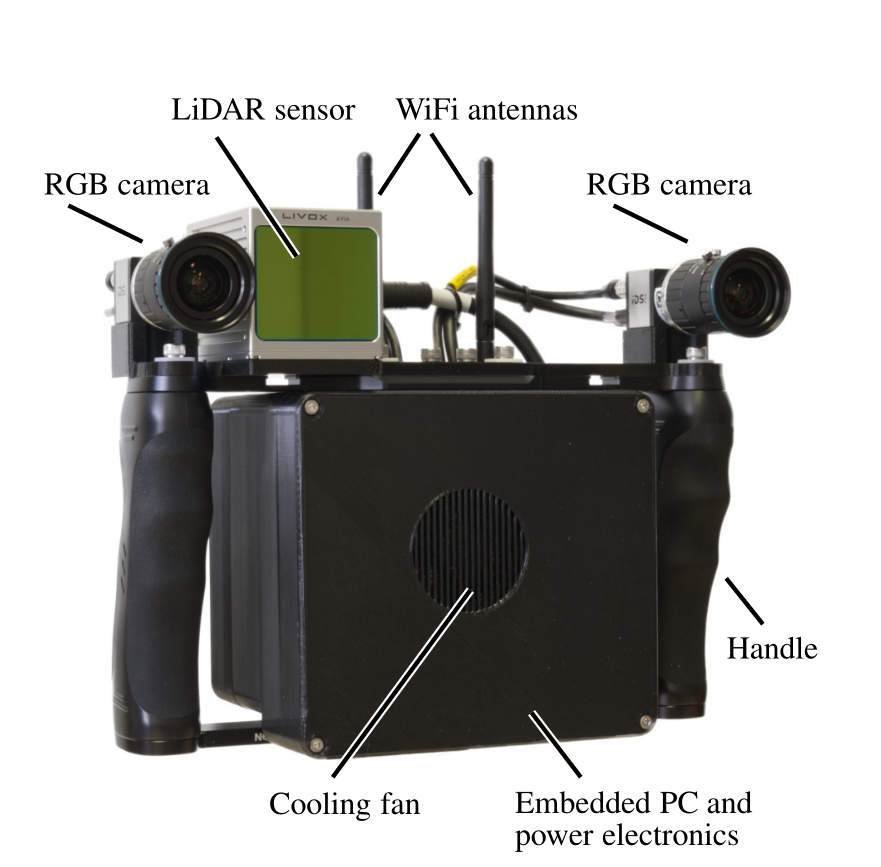
\includegraphics[width=0.8\textwidth]{pics/Handheld_Bleier.png}
    \caption{Handheld stereo vision--LiDAR mapping system featuring stereo cameras, 
    Livox Avia LiDAR, embedded PC, handle and Wi-Fi antenna on a commercial cage rig by Bleier et al.~\cite{bleier2024}}
    \label{fig:bleier_handheld_design}
\end{figure}

\chapter{Theoretical Background}

\section{LiDAR Scanning}
Lidar (Light Detection and Ranging) is a remote sensing technology that measures distances by emitting laser
pulses and recording the time it takes for the reflected signal to return. This time-of-flight measurement
allows precise determination of the distance to an object. Compared to radar, Lidar uses shorter wavelengths,
which makes it more effective for detecting smaller targets. By scanning surfaces, Lidar can also determine
the shape and size of objects, making it highly suitable for terrain modeling and object recognition.
\subsection*{Differential Absorption Lidar (DIAL)}
Differential Absorption Lidar (DIAL) measures atmospheric properties such as temperature, density and
pressure of trace gases and aerosols. It uses two laser beams: one with a wavelength corresponding to the
absorption peak of the target gas (on-line) and another between absorption features (off-line). The ratio
of the returned on-line and off-line signals provides information about the absorption characteristics of
the target gas.
\subsection*{Doppler LiDAR}
Doppler Lidar measures the velocity of targets using the Doppler shift of the reflected light. By mixing
the return signal with a reference laser of known frequency (heterodyne detection), the Doppler frequency
shift can be determined. Applications include wind speed and direction measurements, detection of turbulence
and wake vortices near airports, monitoring local winds during rocket or shuttle launches and providing
data for accurate weather prediction models.

\subsection*{Distance Measurement}
The distance measurement in Lidar follows \( d = \frac{c \cdot t}{2} \), where \(c\) is the speed of light
in vacuum (approximately 299,792,458 m/s) and \(t\) is the pulse time-of-flight. Achieving a resolution of
10 mm requires timing precision on the order of picoseconds (\(10^{-12}\) s). Unlike radar, which emits
diverging signals, Lidar beams are focused. This ensures high accuracy but makes the system sensitive to
fog, rain, wind and reflective or transparent surfaces such as glass or water.

Laser scanners produce raw data that depend on angular resolution (typically 0.25°–1°) and field of view
(commonly 180°, some sensors up to 360°). Raw data generally consist of angle and distance measurements,
optionally including reflectance or intensity. These polar coordinates can be converted to Cartesian
coordinates for further processing and analysis.~\cite{michaelbleier_slides}

\section{PLA -- polylactic acid}
\label{sec:PLA}

PLA, alongside ABS, is one of the most commonly used materials in FDM printers. 
These polylactides are synthetic polymers that belong to the polyester family and are made up of many chemically bonded 
lactic acid molecules. PLA is made from renewable raw materials such as corn starch and is industrially compostable. 

PLA is the material of choice, especially for beginners in 3D printing, as it is forgiving of many printing errors 
and has many other advantages. For example, it can be easily processed by any standard 3D printer, has a low melting 
point and exhibits minimal warping during printing. Furthermore, it is colorfast and scratch-resistant and, unlike ABS, 
produces little odor during processing.~\cite{material4print2024pla}

%\section{\textcolor{red}{IMU -- Inertial Measurment Unit}}

\section{Intrinsic Camera Calibration}
The characteristics of a camera can basically be divided into intrinsic and extrinsic parameters.
Intrinsic calibration captures the camera's internal physical characteristics, such as focal length,
 optical axis, and lens distortion.
Extrinsic calibration, on the other hand, determines the spatial position and orientation of the camera 
relative to a defined world coordinate system.

Intrinsic camera calibration aims to estimate the internal parameters of a camera that model the image 
formation process and lens distortions. According to Fusiello~\cite{Fusiello2024}, this includes focal 
lengths, the principal point and parameters describing lens-induced distortions.

\subsection*{Camera Model}
In the pinhole camera model, a 3D point $\mathbf{X} = [X, Y, Z]^\top$ is projected onto the image 
plane as:
\[
s \begin{bmatrix} u \\ v \\ 1 \end{bmatrix}
= \mathbf{K} \, [\mathbf{I} \mid \mathbf{0}] \,
\begin{bmatrix} X \\ Y \\ Z \\ 1 \end{bmatrix}.
\]
The intrinsic matrix $\mathbf{K}$ is defined as:
\[
\mathbf{K} = 
\begin{bmatrix}
f_x & s & c_x \\
0 & f_y & c_y \\
0 & 0 & 1
\end{bmatrix},
\]
where $f_x$ and $f_y$ are the focal lengths in pixels, $(c_x, c_y)$ is the principal point, and 
$s$ is the skew factor, often assumed to be zero in most practical systems.

\subsection*{Distortion Model}
Real lenses introduce \emph{radial} and \emph{tangential} distortions. A common distortion model with 
radial coefficients $k_1, k_2, k_3$ and tangential coefficients $p_1, p_2$ is:
\[
r^2 = x^2 + y^2,
\]
\[
x_{\mathrm{dist}} = x \left( 1 + k_1 r^2 + k_2 r^4 + k_3 r^6 \right) + 2 p_1 x y + p_2 (r^2 + 2 x^2),
\]
\[
y_{\mathrm{dist}} = y \left( 1 + k_1 r^2 + k_2 r^4 + k_3 r^6 \right) + p_1 (r^2 + 2 y^2) + 2 p_2 x y.
\]
The distorted normalized coordinates $(x_{\mathrm{dist}}, y_{\mathrm{dist}})$ are then mapped to pixel 
coordinates using $\mathbf{K}$.

\subsection*{Calibration Workflow}
Fusiello describes a typical calibration pipeline as follows:
\begin{enumerate}
    \item Capture multiple images (10--20) of a planar calibration target (e.g., checkerboard) from 
          different positions and orientations.
    \item Detect known 2D feature points in the images and associate them with their known 3D coordinates 
          in the target's frame.
    \item Compute an initial estimate of the intrinsic parameters using linear methods (e.g., via 
          homography decomposition).
    \item Refine all intrinsic parameters and distortion coefficients by nonlinear optimization (e.g., 
          Levenberg--Marquardt) to minimize the reprojection error.
\end{enumerate}

\begin{figure}[ht!]
    \centering
    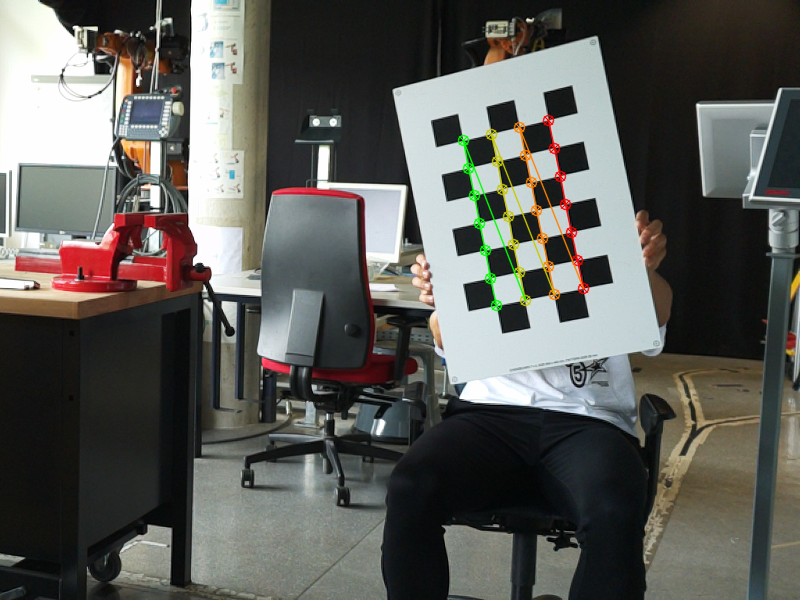
\includegraphics[width=\linewidth]{pics/captured_chessboards/chessboard_005_annotated.png}
    \caption{Example calibration pattern with found corners}
    \label{fig:pattern}   
\end{figure}

%\paragraph{Summary}
%Intrinsic calibration is a fundamental prerequisite for accurate 3D reconstruction and multi-sensor 
%fusion. By estimating the true internal parameters of the camera and compensating for lens distortions, 
%it ensures that image measurements correspond correctly to geometric rays in 3D space.

\section{Extrinsic Calibration of LiDAR and Camera}
\label{sec:extrinsic_calib}

In multi-sensor perception systems that combine LiDAR and camera data, the accurate estimation of the spatial 
relationship between the two sensors is fundamental for enabling sensor fusion. This relationship is described 
by a rigid-body transformation that maps coordinates from the LiDAR reference frame into the camera reference frame. 
If this transformation is incorrect, the projected LiDAR points will not align with the corresponding image features, 
leading to degraded performance in tasks such as 3D reconstruction, object detection or semantic segmentation. 
Extrinsic calibration aims to estimate this transformation with high precision. The approach described in~\cite{beltran2022automatic} 
achieves this in a fully automated manner, without the need for dedicated calibration targets, making it applicable in a wide variety 
of real-world scenarios.

Formally, let $\mathcal{L}$ denote the LiDAR coordinate frame and $\mathcal{C}$ the camera coordinate frame. 
The calibration problem consists of finding the homogeneous transformation matrix $\mathbf{T}_{\mathcal{CL}} \in SE(3)$ that maps a 
point $\mathbf{p}_L$ expressed in LiDAR coordinates to its representation $\mathbf{p}_C$ in the camera coordinate system:
\begin{equation}
\mathbf{p}_C =
\mathbf{T}_{\mathcal{CL}} \, \mathbf{p}_L
= \begin{bmatrix} \mathbf{R} & \mathbf{t} \\ \mathbf{0}^\top & 1 \end{bmatrix} \mathbf{p}_L,
\label{eq:extrinsic_transformation}
\end{equation}
where $\mathbf{R} \in SO(3)$ is a rotation matrix and $\mathbf{t} \in \mathbb{R}^3$ is a translation vector. 
This transformation describes both the orientation and the position of the LiDAR relative to the camera. 
The points $\mathbf{p}_L$ are represented in homogeneous coordinates, enabling both rotation and translation to be applied in a single 
matrix multiplication.

Once a LiDAR point has been transformed into the camera coordinate frame, it is projected into the image plane using the calibrated pinhole camera model. 
This projection is given by:
\begin{equation}
\mathbf{u} \sim \mathbf{K} \, [\mathbf{R} \;|\; \mathbf{t}] \, \mathbf{p}_L,
\label{eq:projection}
\end{equation}
where $\mathbf{K}$ is the intrinsic camera matrix containing focal lengths, the principal point, and skew parameters, and $\mathbf{u} = [u, v, 1]^\top$ are 
the homogeneous image coordinates. The operator $\sim$ indicates equality up to a scale factor due to the use of homogeneous coordinates. Accurate knowledge 
of $\mathbf{K}$ is assumed, as intrinsic calibration is typically performed separately beforehand.

The extrinsic calibration problem can then be formulated as an optimization that minimizes the discrepancy between the observed image features and the 
projections of the corresponding LiDAR points. This is expressed as the minimization of the total reprojection error:
\begin{equation}
E(\mathbf{R}, \mathbf{t}) =
\sum_{i=1}^N \left\| \mathbf{u}_i -
\pi\left( \mathbf{R} \mathbf{p}_{L,i} + \mathbf{t} \right) \right\|^2,
\label{eq:reprojection_error}
\end{equation}
where $\pi(\cdot)$ is the projection function defined in Equation~\ref{eq:projection}, $\mathbf{u}_i$ are observed feature points in the image, and $\mathbf{p}_{L,i}$ 
are the corresponding 3D points from the LiDAR point cloud. The summation is performed over $N$ matched feature correspondences. By minimizing $E$, the algorithm ensures 
that the transformed and projected LiDAR points align as closely as possible with the observed image features.

The automated calibration procedure proceeds through several interconnected stages, each of which plays a crucial role in the accuracy and robustness of the final result. 
The first stage consists of data acquisition. The system records synchronized LiDAR point clouds and camera images from a variety of viewpoints within the target environment. 
Multiple poses and viewing angles are necessary to provide the optimization with a rich set of correspondences and to reduce
degeneracy in the solution, particularly in geometrically uniform scenes.
The second stage is feature extraction. In the image domain, this often involves detecting salient structures such as edges, corners or line segments that are stable 
under viewpoint changes and can be reliably localized. In the LiDAR domain, geometric primitives such as planes, sharp edges or high-intensity reflectors are extracted 
from the 3D point cloud. These features should ideally correspond to physical elements in the scene that are visible to both sensors, such as building edges, traffic signs
or corners of large objects.

The third stage is feature association. This is a challenging problem because LiDAR and camera sensors capture different modalities: LiDAR measures geometry and sometimes 
reflectivity, while cameras measure color and intensity. To establish correspondences, the algorithm projects candidate LiDAR features into the image using a tentative 
transformation and searches for spatially consistent matches with the extracted image features. Similarity measures can be based on geometric alignment, intensity patterns 
or mutual visibility constraints. At this point, only approximate correspondences are needed, as they will be refined later.

Once a sufficient set of correspondences is established, the fourth stage computes an initial estimate of the transformation $\mathbf{T}_{\mathcal{CL}}$. 
If direct 3D -- 3D correspondences between LiDAR and camera coordinate frames are available -- such as from triangulated stereo image points -- this estimate can be obtained in 
closed form using the Kabsch algorithm, which minimizes the root-mean-square distance between matched point sets. If only 3D–2D correspondences are available, 
a Perspective-n-Point (PnP) algorithm can be employed to obtain an initial rotation and translation.

The fifth stage refines the transformation through nonlinear optimization. Here, the initial $(\mathbf{R}, \mathbf{t})$ is used as a starting point for minimizing the 
reprojection error defined in Equation~\ref{eq:reprojection_error}. The optimization is typically carried out using the Levenberg–Marquardt algorithm, which is well 
suited for nonlinear least-squares problems. Robust loss functions, such as the Huber or Cauchy loss, are integrated into the cost function to reduce the influence of 
outlier correspondences that could arise from incorrect feature matches or transient objects in the scene.

Finally, the sixth stage is validation. The estimated transformation is applied to the LiDAR point cloud, and the points are projected into the corresponding camera image. 
Visual inspection can reveal any systematic misalignment, while quantitative measures such as the mean or median reprojection error provide objective performance metrics. 
Figures~\ref{fig:steps}, \ref{fig:detect_extrinsic_calib} and \ref{fig:reprojection} illustrate the calibration pipeline, the involved coordinate frames and an example of a calibrated projection.

This fully automated pipeline offers several advantages. By eliminating the need for artificial calibration targets, it can be executed in natural, dynamic environments 
without disrupting regular operation. Its reliance on common scene features rather than engineered markers makes it flexible across domains, from autonomous driving and 
mobile robotics to large-scale 3D mapping. At the same time, the combination of an initial analytical estimate with a robust nonlinear refinement ensures both convergence 
reliability and high final accuracy.

\begin{figure}[htbp]
    \centering
    % Erste Reihe
    \begin{subfigure}[b]{0.45\textwidth}
        \centering
        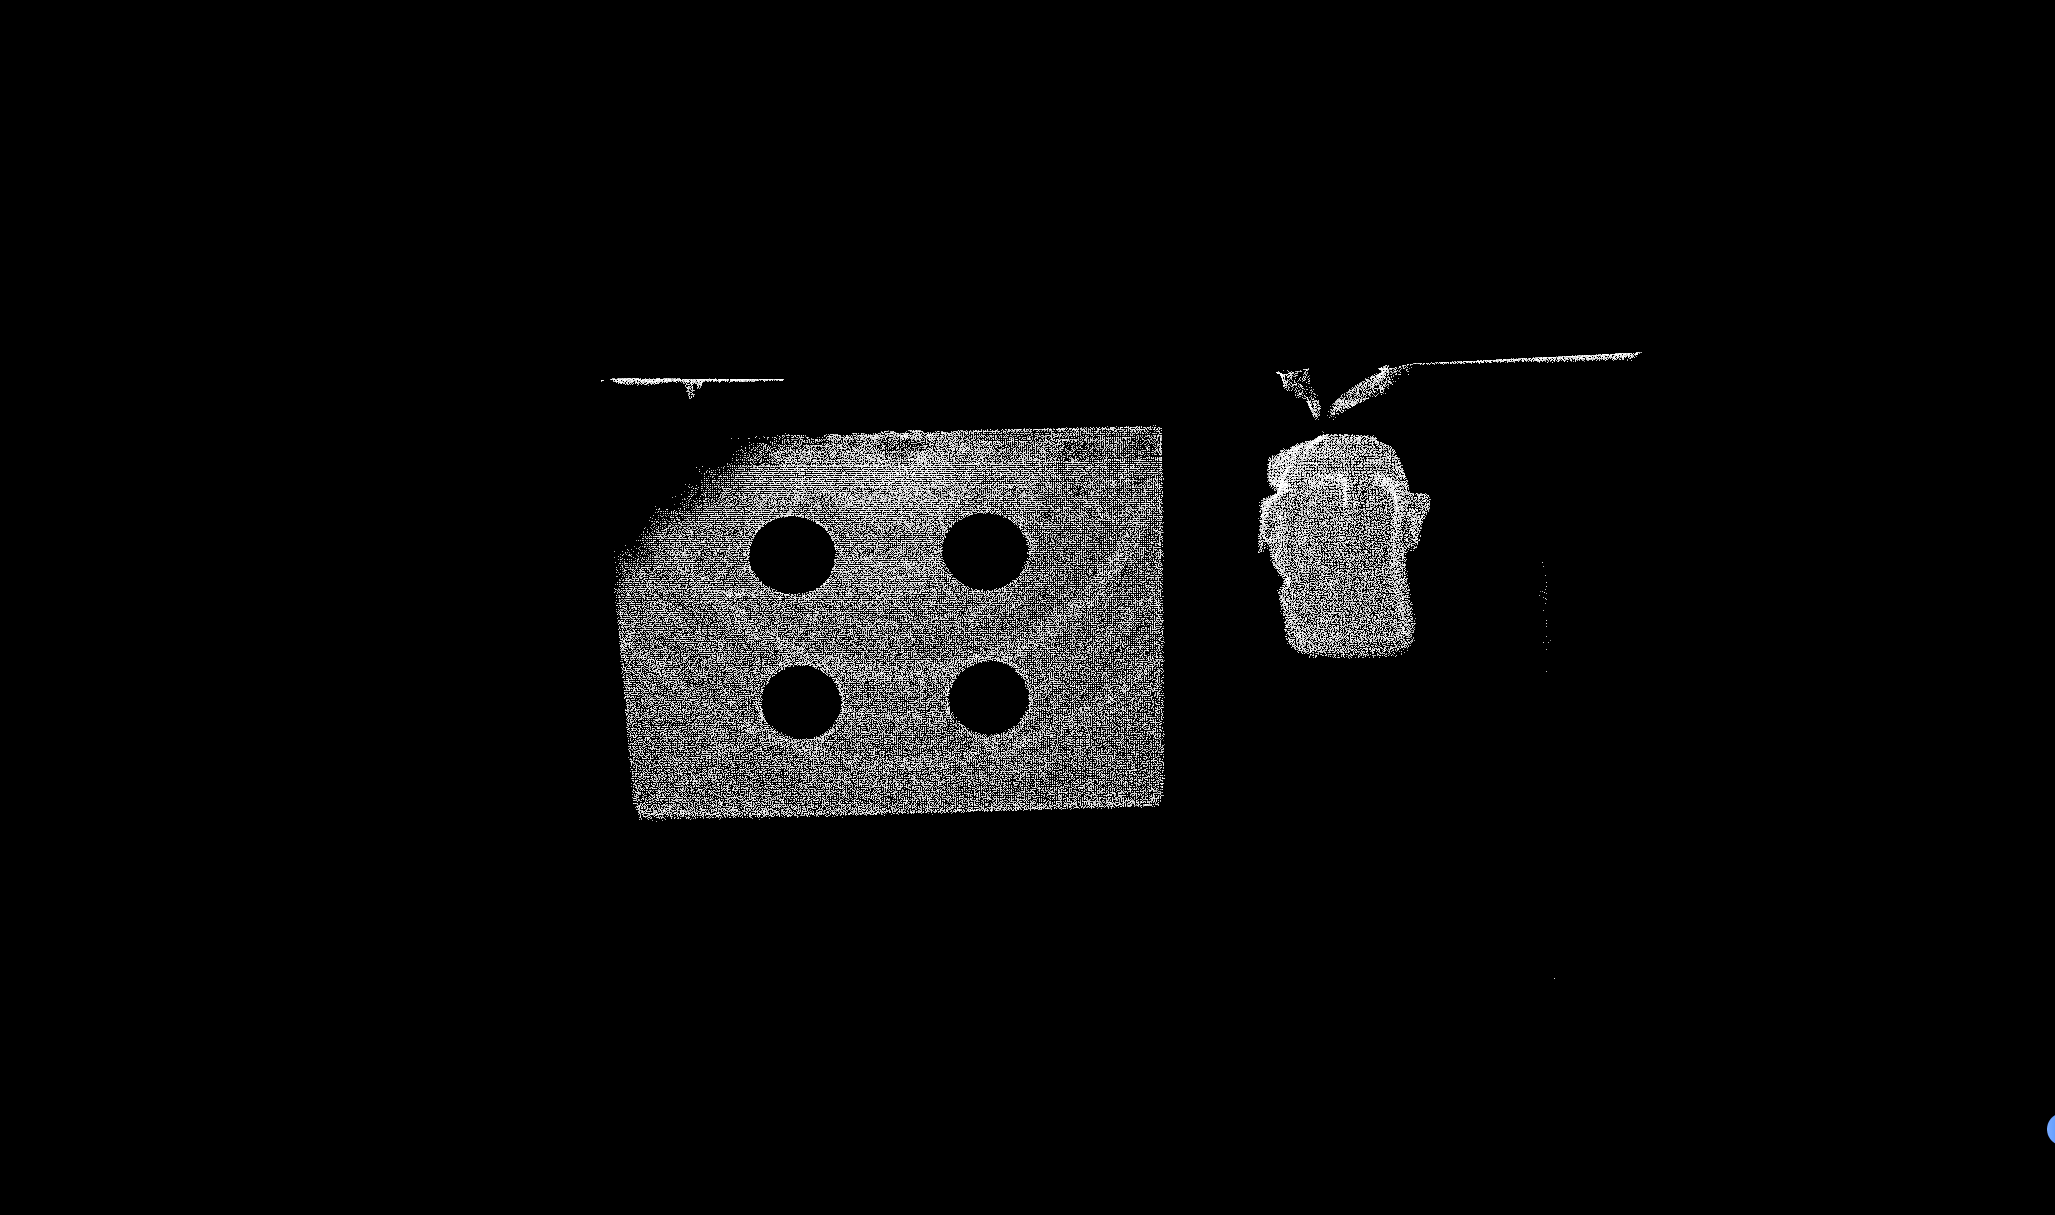
\includegraphics[width=\linewidth]{pics/calib_pics/filter.png}
        \caption{Step 1: Distance Filtering}
    \end{subfigure}
    \hfill
    \begin{subfigure}[b]{0.45\textwidth}
        \centering
        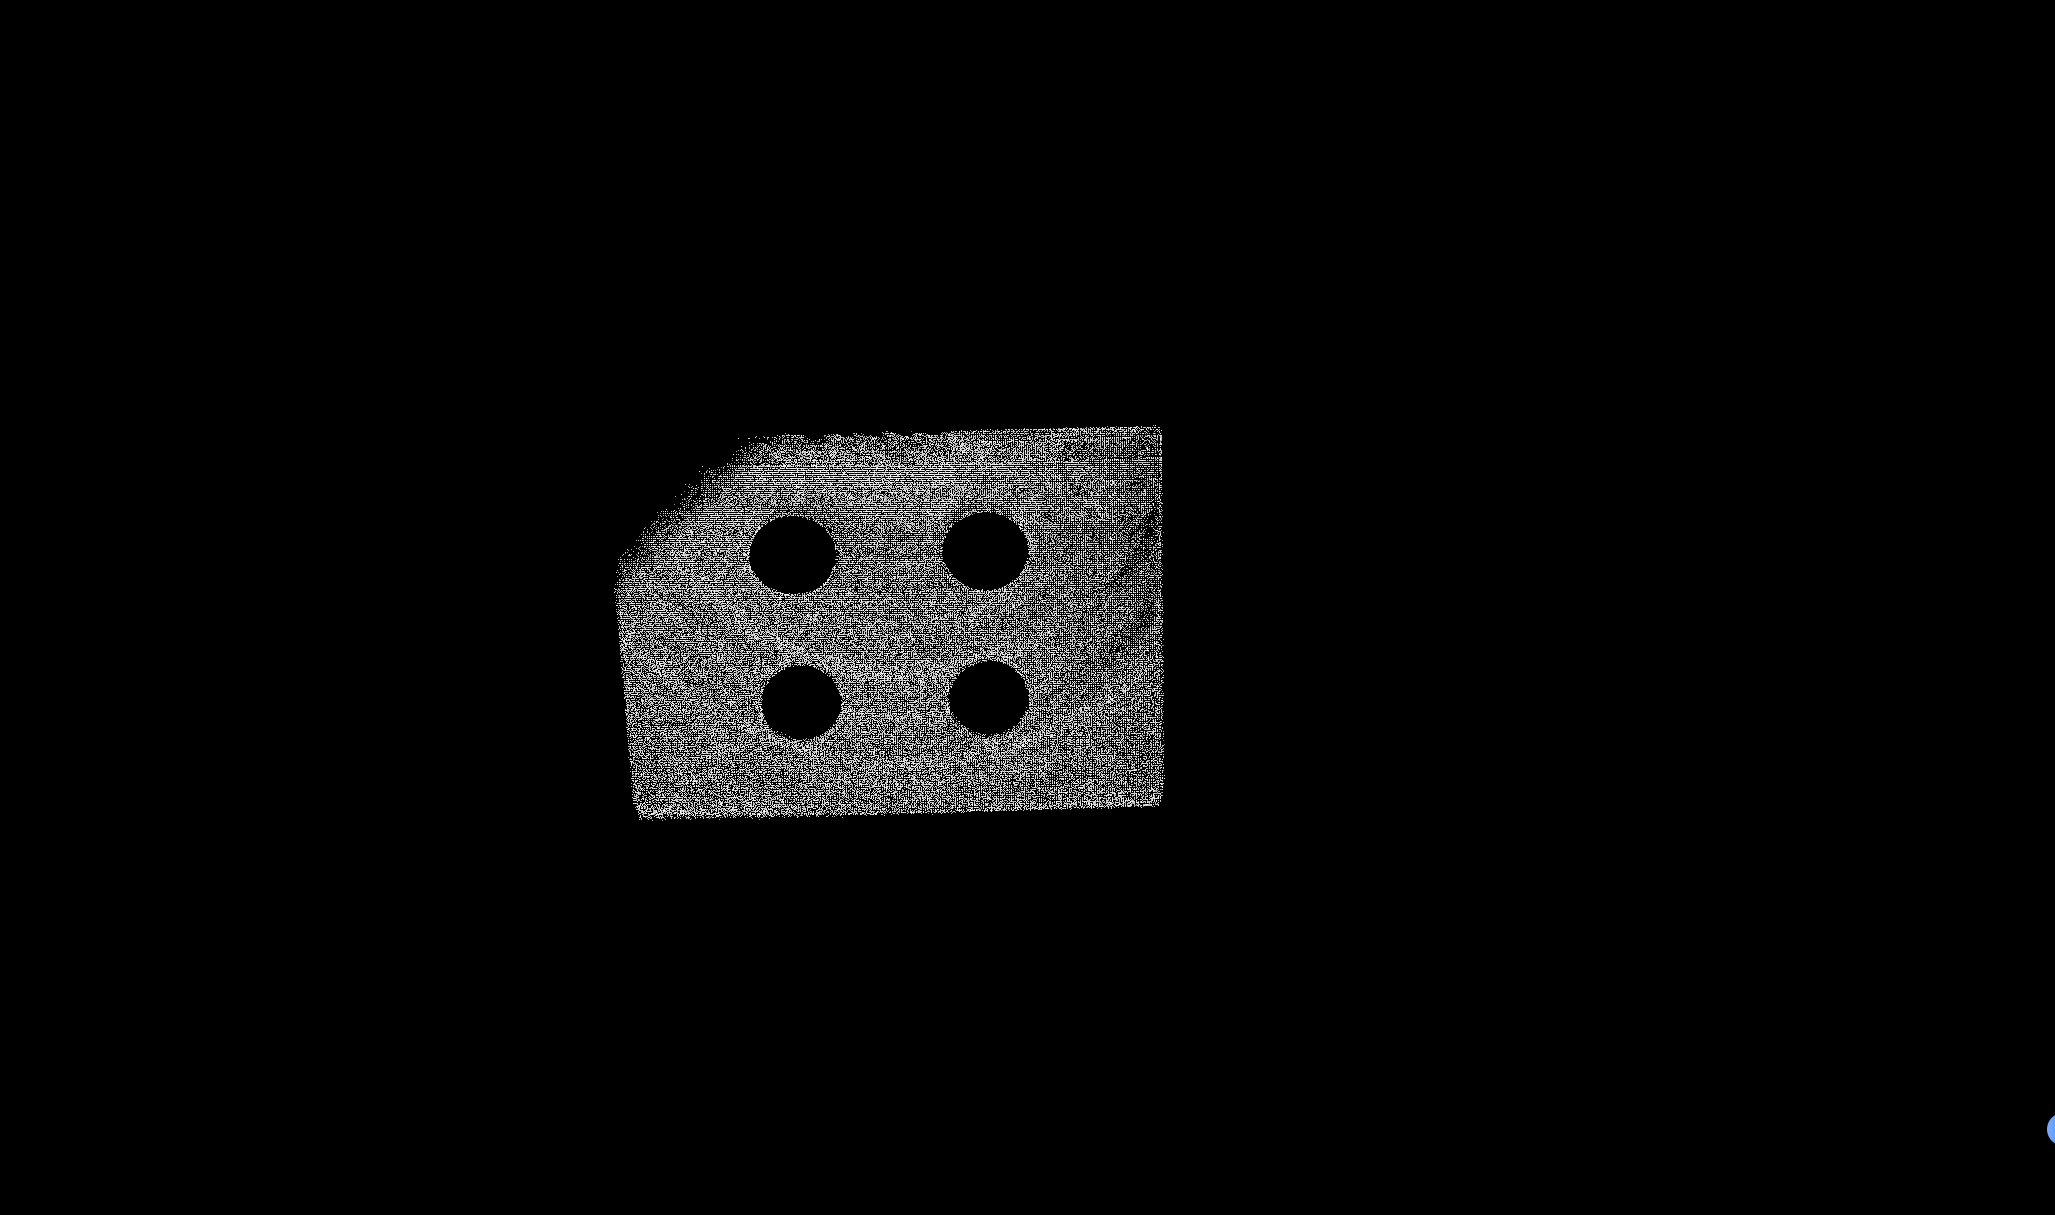
\includegraphics[width=\linewidth]{pics/calib_pics/plane.png}
        \caption{Step 2: Plane Segmentation}
    \end{subfigure}

    % Zweite Reihe
    \begin{subfigure}[b]{0.45\textwidth}
        \centering
        
\includegraphics[width=\linewidth]{pics/calib_pics/aligned.png}
        \caption{Step 3: Plane Alignment to 2D}
    \end{subfigure}
    \hfill
    \begin{subfigure}[b]{0.45\textwidth}
        \centering
        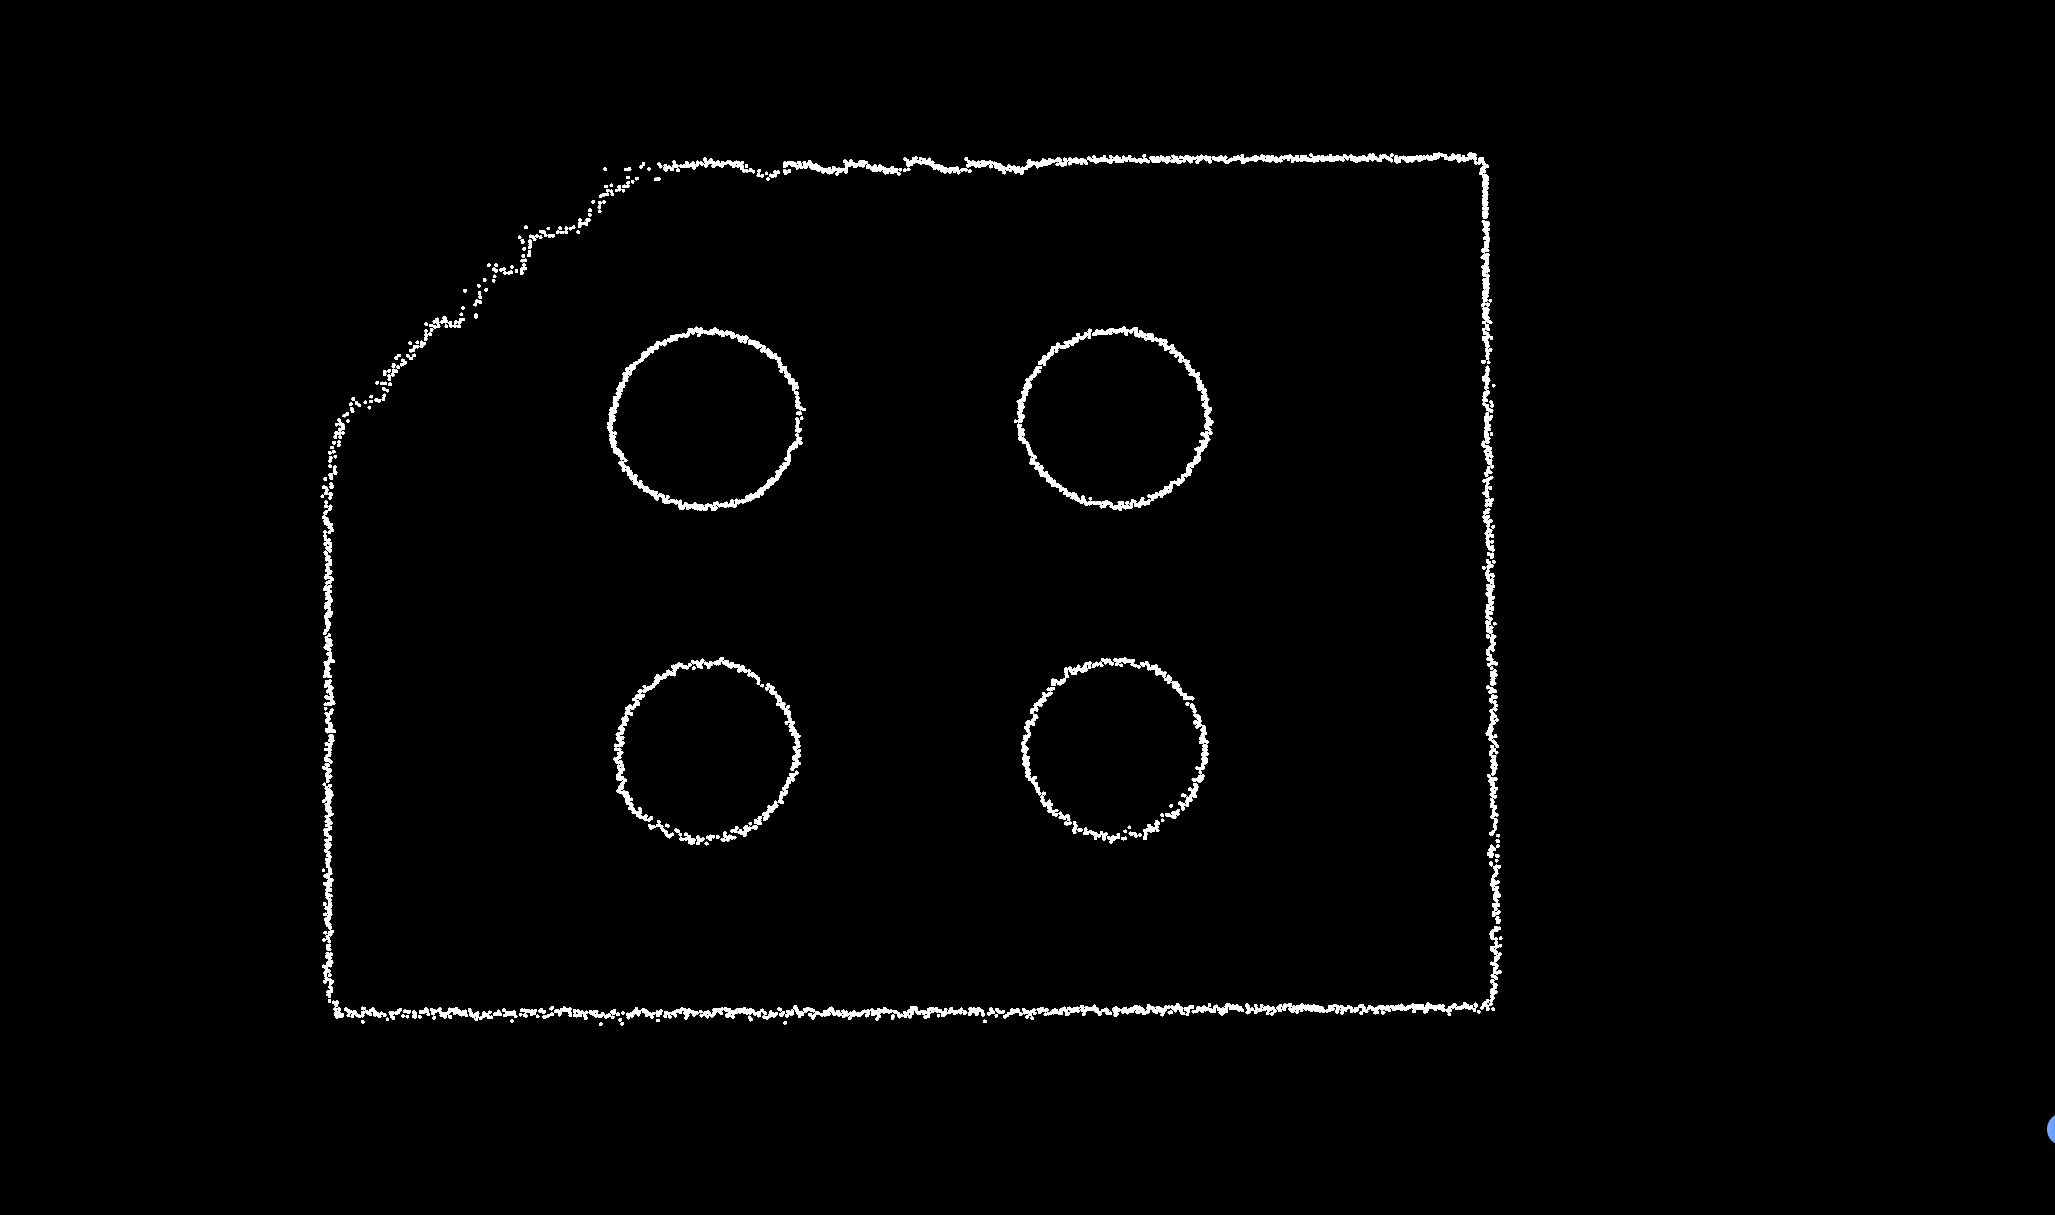
\includegraphics[width=\linewidth]{pics/calib_pics/edge.png}
        \caption{Step 4: Boundary Point Detection}
    \end{subfigure}

    % Dritte Reihe
    \begin{subfigure}[b]{0.45\textwidth}
        \centering
        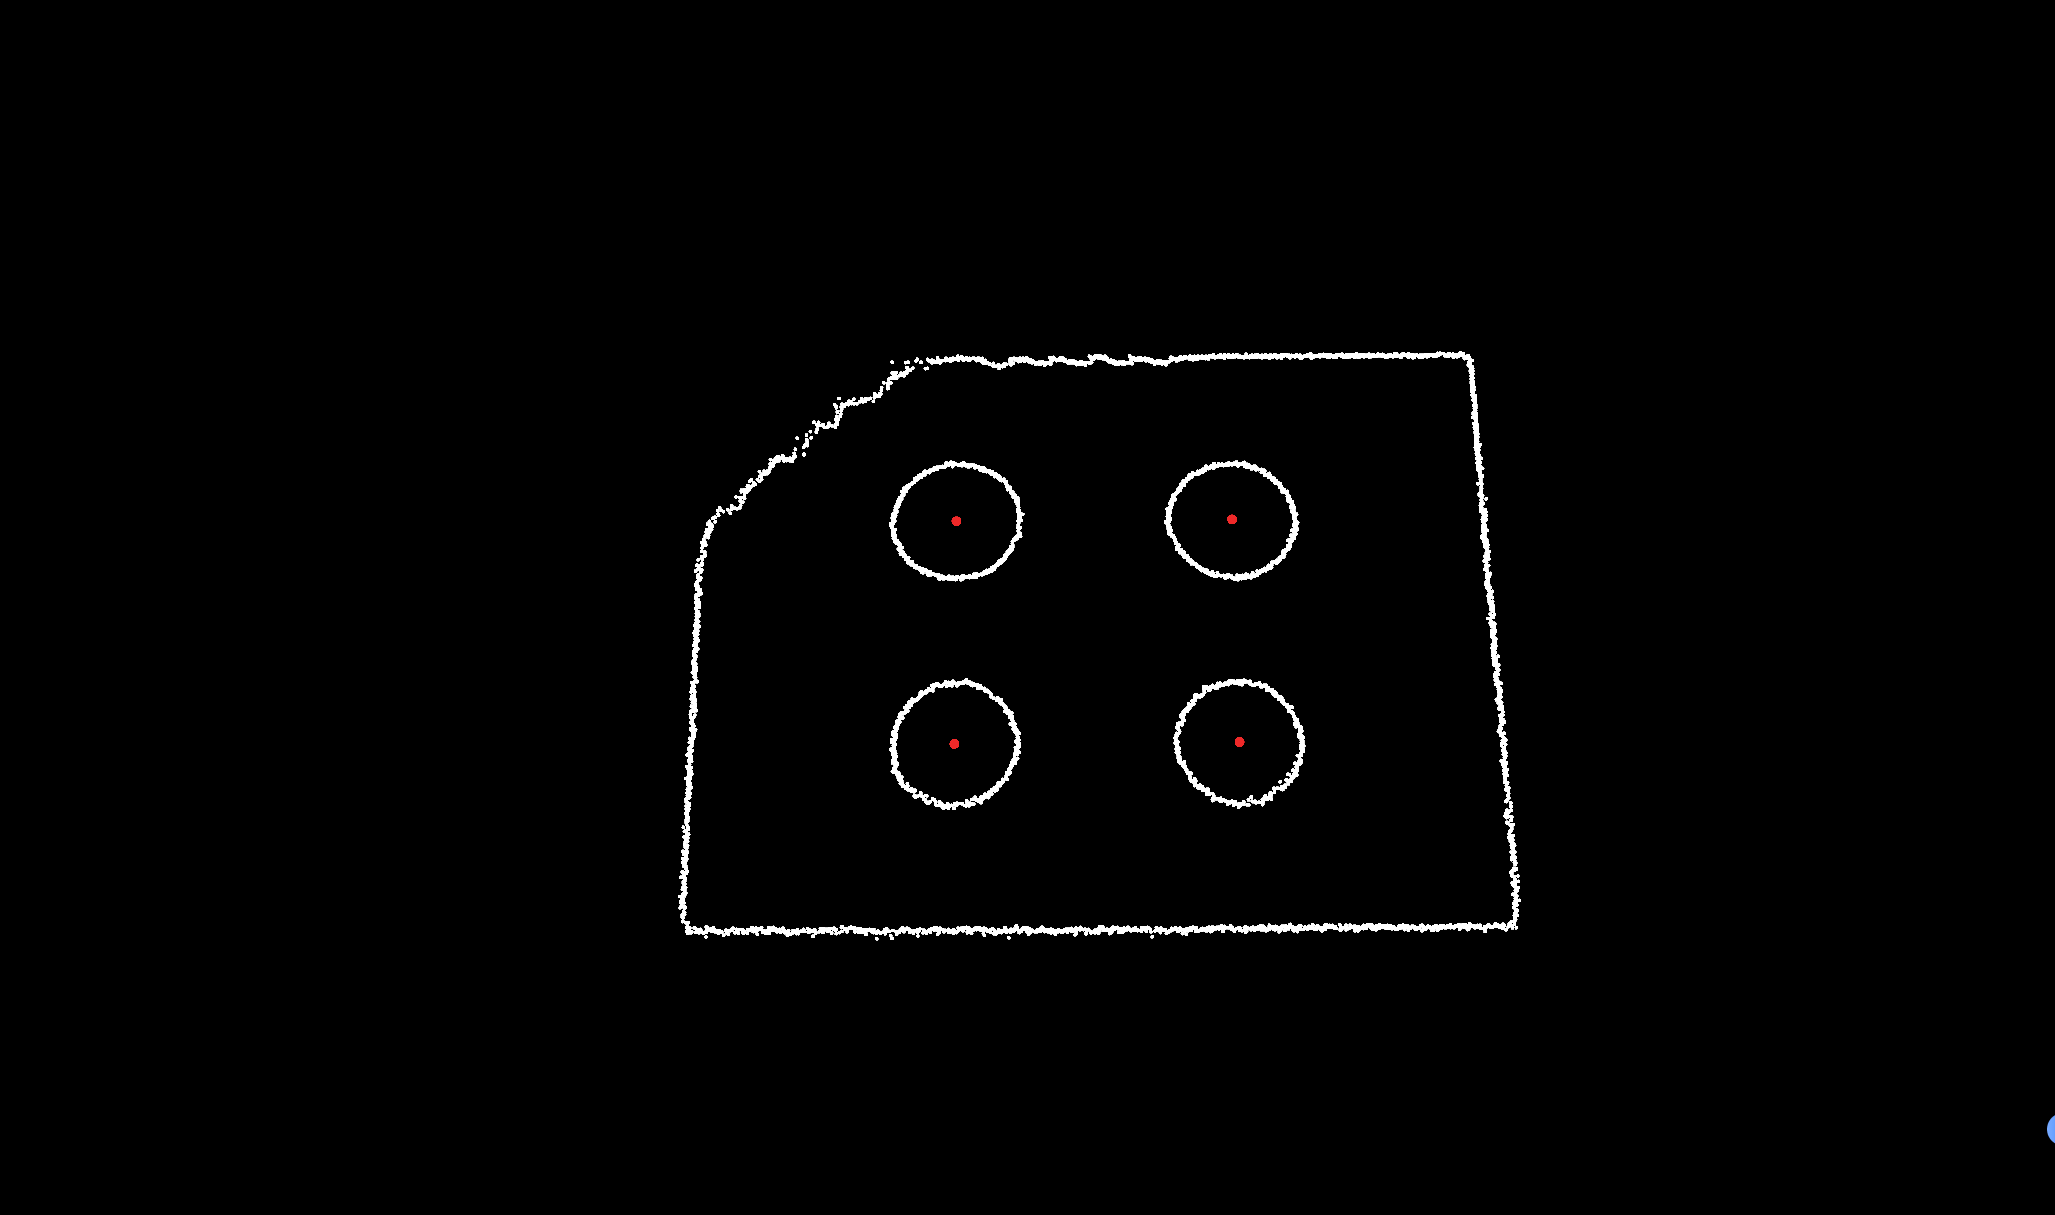
\includegraphics[width=\linewidth]{pics/calib_pics/cluster.png}
        \caption{Step 5: Clustering and Circle Fitting}
    \end{subfigure}
    \hfill
    \begin{subfigure}[b]{0.45\textwidth}
        \centering
        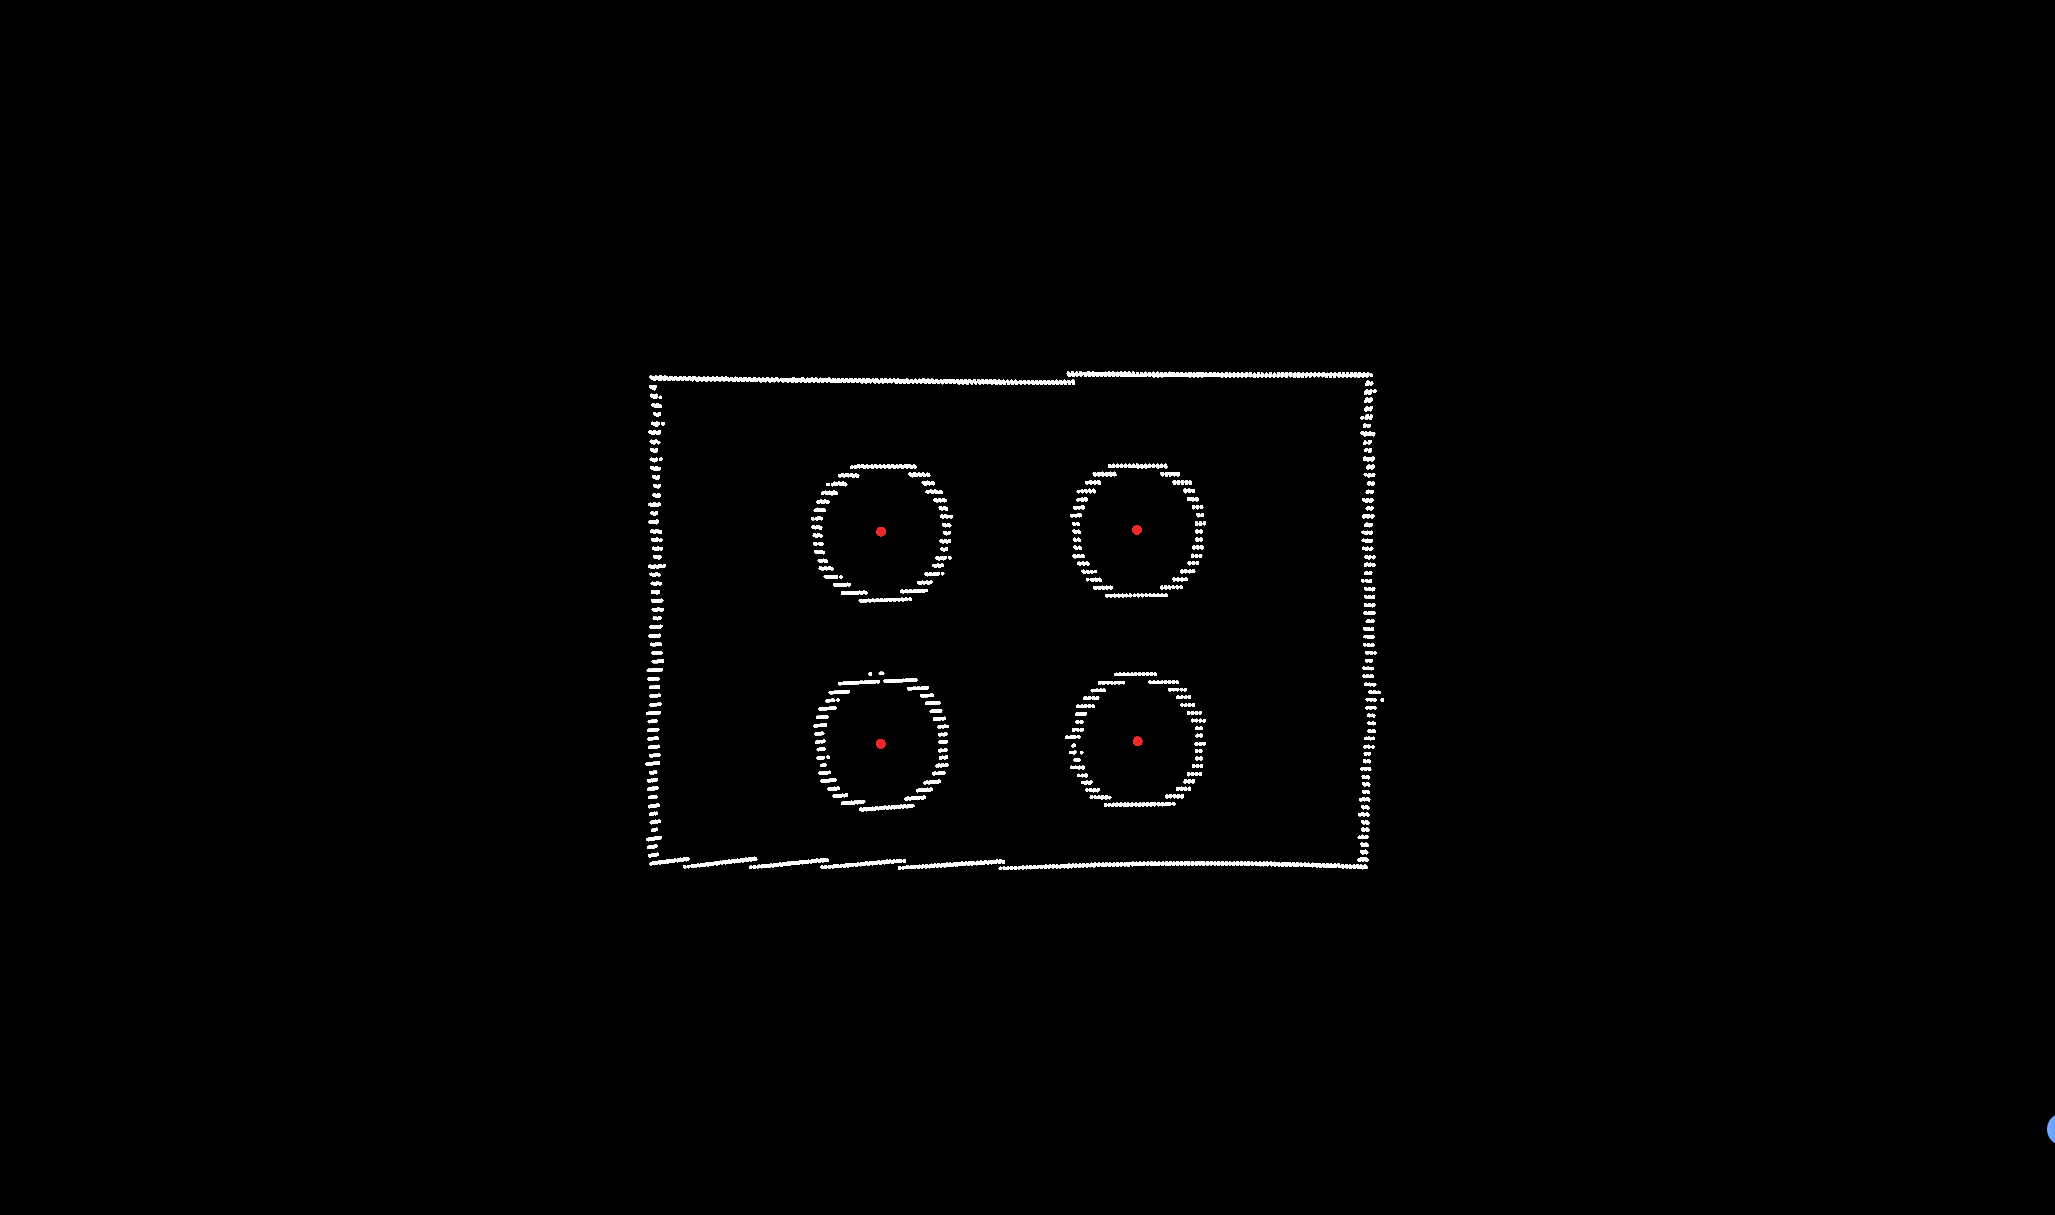
\includegraphics[width=\linewidth]{pics/calib_pics/ouster_cluster.png}
        \caption{Step 6: Performance of LiDAR}
    \end{subfigure}

    \caption{LiDAR--camera extrinsic calibration pipeline\cite{FASTCalibROS2}}
    \label{fig:steps}
\end{figure}

\begin{figure}[ht!]
    \centering
    %coordinate_frames.png
    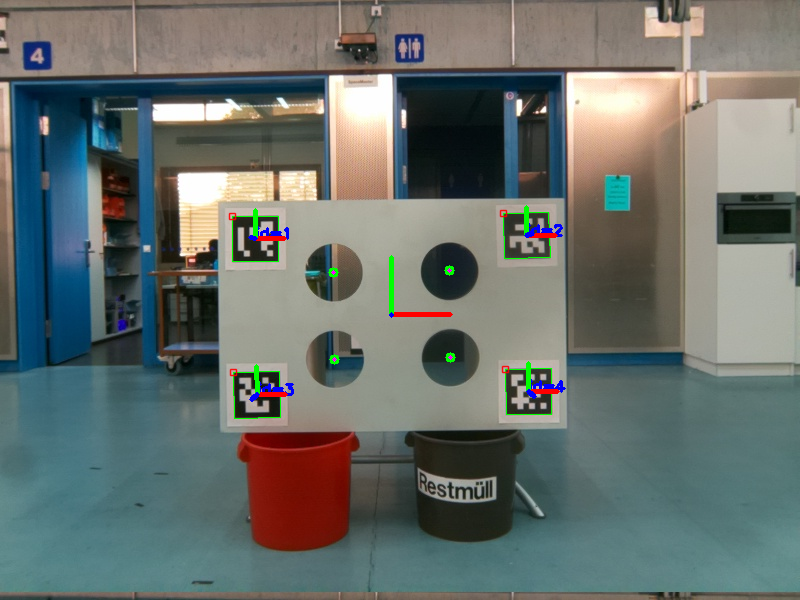
\includegraphics[width=0.7\linewidth]{pics/qr_detect_robo.png}
    \caption{Detected calibration pattern}
    \label{fig:detect_extrinsic_calib}
\end{figure}

\begin{figure}[ht!]
    \centering
    %reprojection_example.png
    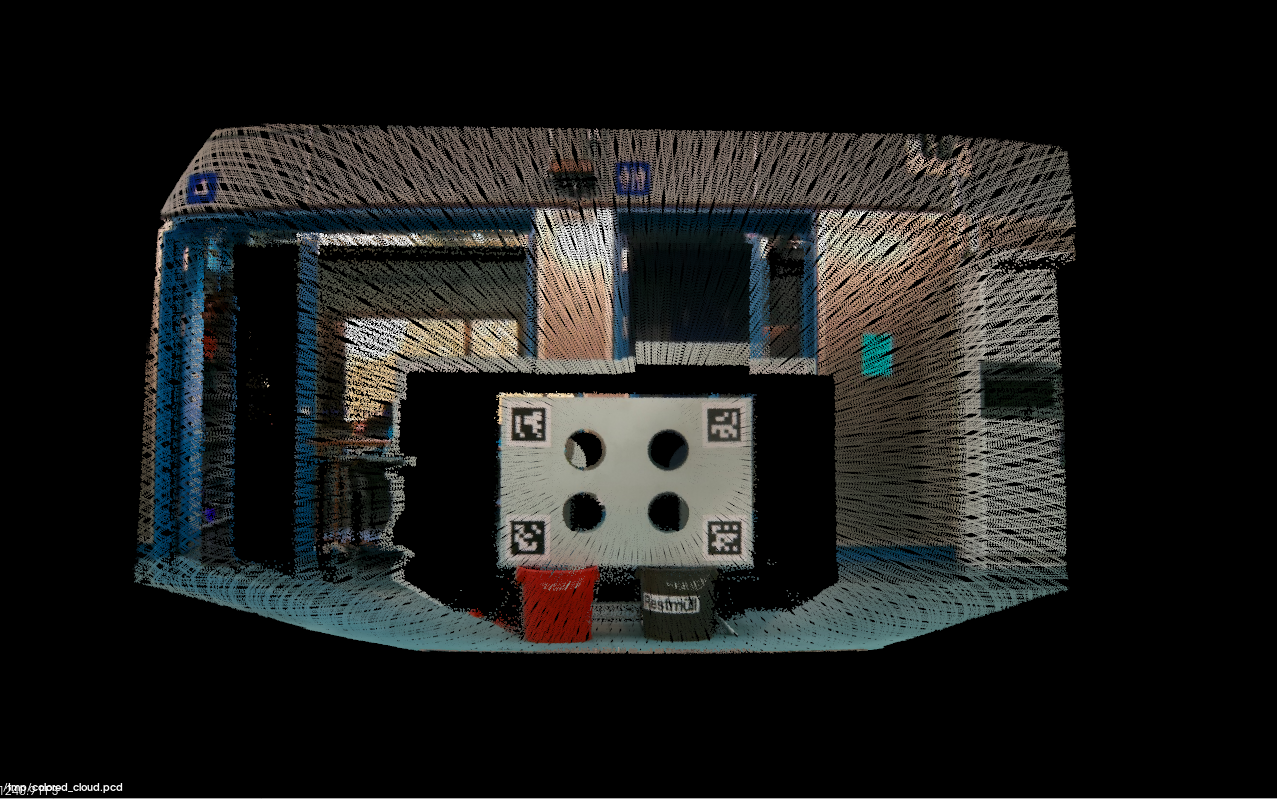
\includegraphics[width=0.7\linewidth]{pics/extrinsic_calib_global.png}
    \caption{Colored pointcloud of FastCalib}
    \label{fig:reprojection}
\end{figure}

    
\section{Synchronize timestamps}
\label{sec:PTP}
In order to correlate the different sensor data from LiDAR, camera and IMU,
i.e., which scan matches which image and what the position was at that time,
we need to synchronize the sensor systems in terms of time.
We use PTP to enable this time synchronization.

The Precision Time Protocol (PTP) according to IEEE~1588 is used for high-precision
synchronization of clocks in distributed systems via packet-based
networks. The architecture is hierarchical and based on
the selection of a \emph{Grandmaster Clock} as a reference clock, whose
time base is adopted by all other participants (\emph{Slaves}).
The grandmaster is determined using the \emph{Best Master
Clock Algorithm} (BMCA), which is based on defined quality parameters of the
respective clocks.
We designate the Raspberry PI as our grandmaster and the connected 
sensors -- LiDAR, camera, and IMU -- as slaves.~\cite{eidson2002ieee}

Synchronization is achieved by exchanging defined messages.
The master sends a
\texttt{Sync} message with a high-resolution timestamp $T_1$ at regular intervals. The
slave records the time of receipt as $T_2$. To determine the
transmission delay, the slave sends a
\texttt{Delay\_Req} message, whose transmission time $T_3$ it records itself.
The master records the time of receipt as $T_4$ and transmits
this in a \texttt{Delay\_Resp} message to the slave.~\cite{wikipediaPTP}

The transmission delay
(one-way delay) is first calculated from the four timestamps:
\[
\text{Delay} = \frac{(T_2 - T_1) + (T_4 - T_3)}{2}
\]
The time offset between the slave and master clocks is calculated as follows:
\[
\text{Offset} = \frac{(T_2 - T_1) - (T_4 - T_3)}{2}
\]
By correcting for the calculated offset, the slave clock can be set precisely to
the time of the master.~\cite{hpePTP}
Accuracy is significantly influenced by the recording of time stamps. 
With software timestamping, this is done at the
protocol level, which can lead to higher jitter values. The
hardware timestamping that we use in our case sets time stamps 
directly in the network interface (MAC/PHY) and enables accuracies in the 
sub-microsecond to nanosecond range.~\cite{wikipediaPTP}

In more complex networks boundary clocks and
transparent clocks are used. Boundary clocks synchronize
with the grandmaster and pass the time on to downstream segments.
 Transparent clocks measure the propagation delay within
a device and include this information in PTP messages to
compensate for runtime errors.~\cite{eidson2002ieee}

The precision depends on the stability of the grandmaster clock, the
symmetry of the transmission paths, the buffer architecture in intermediate nodes
and the accuracy of the time stamping. Under optimal conditions,
 hardware timestamping can achieve accuracies in the nanosecond range.~\cite{hpePTP}

Since in our setup (\ref{fig:Master_Slave}) only the laser scanner is connected to the Pi via Ethernet
and the camera and IMU are connected directly to the Pi via CSI and I2C, respectively,
and therefore already run under Raspberry--Pi Time, we only need to synchronize the Livox.
This is the case because the Livox Mid-70 produces its own timestamps by default, 
which simply indicate the time that has elapsed since the start
of the laser scanner.

To solve the synchronization task, we use PTP daemon (PTPd).

\begin{figure}[h!]
    \centering
    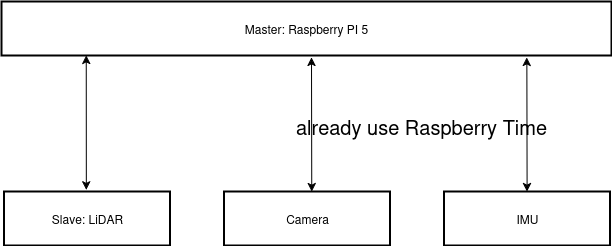
\includegraphics[width=\textwidth]{pics/Master_Slave.png}
    \caption{Time synchronization pipeline}
    \label{fig:PTP}
\end{figure}

\begin{figure}[h!]
    \centering
    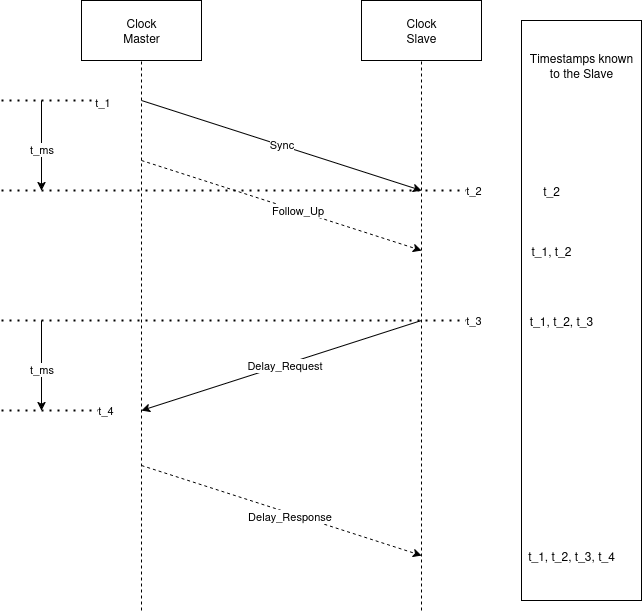
\includegraphics[width=\textwidth]{pics/PTP.png}
    \caption{PTP synchronization between slave and master\cite{wikipediaPTP}}
    \label{fig:Master_Slave}
\end{figure}


\section{Projection from LiDAR to Image space}
\label{sec:proj_lidar_image}
The projection of LiDAR points into an image frame is a fundamental step for multi-sensor fusion. 
Given a point $\mathbf{P}_L = [X_L, Y_L, Z_L, 1]^\top$ expressed in the LiDAR coordinate system, 
the transformation into the camera coordinate system is defined by a rigid-body motion:
\[
  \mathbf{P}_C = \mathbf{R}\,\mathbf{P}_L + \mathbf{t},
\]
where $\mathbf{R} \in SO(3)$ is the rotation matrix describing the orientation of the LiDAR relative 
to the camera, and $\mathbf{t} \in \mathbb{R}^3$ is the translation vector. Together they form the 
extrinsic calibration parameters, which encode the spatial relationship between both sensors 
\cite{mishra2020extrinsic}.

Once the 3D point is represented in the camera frame $\mathbf{P}_C = [X_C, Y_C, Z_C]^\top$, it can 
be mapped into the 2D image plane using the pinhole camera model:
\[
  \lambda
  \begin{bmatrix}
  u \\ v \\ 1
  \end{bmatrix}
  =
  \mathbf{K}
  \begin{bmatrix}
  X_C \\ Y_C \\ Z_C
  \end{bmatrix},
\]
with $\mathbf{K}$ denoting the intrinsic matrix and $(u,v)$ representing the pixel coordinates. 
Here $\lambda$ corresponds to the projective depth $Z_C$, ensuring that the normalized coordinates 
are obtained as
\[
  u = \frac{f_x X_C}{Z_C} + c_x, \quad v = \frac{f_y Y_C}{Z_C} + c_y,
\]
where $(f_x,f_y)$ denote the focal lengths in pixel units and $(c_x,c_y)$ are the principal point 
coordinates \cite{review2024lidarcamera}.

In practice, only points with $Z_C > 0$ are retained, since negative depths correspond to locations 
behind the camera plane. Furthermore, projected coordinates must lie within the valid image bounds, 
otherwise they are discarded. This ensures that the resulting projection covers only the visible 
region of the image and allows one to verify whether the LiDAR field of view fully overlaps with the 
camera’s image space. The described implementation corresponds directly to the function 
\texttt{project\_lidar\_on\_image}, which applies the extrinsic transformation, projects the points 
through the intrinsic matrix and renders them as overlay positions on the RGB image.

%\begin{figure}[H]
%    \centering
%    \includegraphics[width=0.7\textwidth]{Platzhalter.jpg}
%    \caption{LiDAR point cloud in 3D space.}
%    \label{fig:lidar_3d_cloud}
%\end{figure}

%\begin{figure}[H]
%    \centering
%    \includegraphics[width=0.7\textwidth]{Platzhalter.jpg}
%    \caption{Projection of LiDAR points into the 2D image plane.}
%    \label{fig:lidar_projection}
%\end{figure}

%\begin{figure}[H]
%    \centering
%    \includegraphics[width=0.7\textwidth]{Platzhalter.jpg}
%    \caption{Overlay of projected LiDAR points on the RGB frame.}
%    \label{fig:lidar_overlay}
%\end{figure}


\section{ICP -- Iterative Closest Point}
The Iterative Closest Point (ICP) algorithm is a widely used technique in computer vision and robotics for rigidly 
aligning two 3D point clouds, typically denoted as a source point set $\mathcal{P} = \{p_i\}_{i=1}^N$ and a target point 
set $\mathcal{Q} = \{q_j\}_{j=1}^M$~\cite{Zhang2016}. The fundamental objective of ICP is to find the optimal rigid 
transformation, consisting of a rotation matrix $R \in SO(3)$ and a translation vector $t \in \mathbb{R}^3$, that minimizes 
the distance between corresponding points in the two sets. Formally, the error metric commonly minimized is the mean 
squared distance:

\[
E(R, t) = \frac{1}{N} \sum_{i=1}^{N} \| R p_i + t - q_{\sigma(i)} \|^2,
\]
where $\sigma(i)$ denotes the index of the closest point in $\mathcal{Q}$ corresponding to $p_i$ in $\mathcal{P}$. The ICP 
algorithm proceeds iteratively, typically following two main steps:

1. **Correspondence Assignment**: For each point $p_i$ in the source set $\mathcal{P}$, the closest point $q_{\sigma(i)}$ 
in the target set $\mathcal{Q}$ is determined, often using Euclidean distance. This step establishes a provisional mapping 
between the point sets.

2. **Transformation Estimation**: Given the correspondences, the optimal rigid transformation $(R^*, t^*)$ is computed by 
minimizing the objective function $E(R, t)$. Closed-form solutions exist for this step, for example using singular value 
decomposition (SVD) of the covariance matrix between the corresponding points.

These steps are repeated iteratively: after applying the computed transformation to the source points, correspondences are 
re-evaluated and a new transformation is estimated. The iteration continues until convergence, which is typically defined 
as the point where the change in the error function $E(R, t)$ between successive iterations falls below a predefined 
threshold.  

Variants of the ICP algorithm enhance its robustness to noise, outliers, and partial overlaps. For instance, weighted ICP 
assigns confidence weights $w_i$ to each correspondence, modifying the error function to:

\[
E_w(R, t) = \frac{1}{\sum_i w_i} \sum_{i=1}^{N} w_i \| R p_i + t - q_{\sigma(i)} \|^2,
\]
while robust error metrics, such as the Huber or Tukey loss, can reduce the influence of outliers. These extensions make 
ICP applicable to a wide range of practical problems in 3D computer vision, robotics mapping, and pose estimation~\cite{Zhang2016}. 

\chapter{Hardware and Design}
\section{Design}

For the design (Figure~\ref{fig:handheld_device}), inspiration was taken from the handheld system 
described in \textit{A handheld stereo vision and LiDAR system for outdoor dense RGB-D mapping 
using depth map completion based on learned priors}~\cite{bleier2024}. Both the LiDAR sensor and 
the monocular camera are mounted on a rectangular box that also houses the essential electronic 
components, including the Raspberry~Pi, the IMU and the DC-DC converter. This compact integration 
ensures that the hardware is mechanically stable and protected against external influences. The 
most notable difference compared to the design presented in \cite{bleier2024} is the integration of 
a battery box, which in this prototype is repurposed from a portable light box. This modification 
enables self-sufficient operation in outdoor environments and highlights the emphasis on 
time-efficient and practical design choices.
A touchscreen was also installed in
the device, which can be used to start recording rosbags and control data acquisition. The display runs
the normal Ubuntu interface, which means that any other action can also be performed on it. Since the device is
still in development, the components and cables have been installed in a very pragmatic way, so that each component
is still easily accessible and cable connections can be checked very quickly without having to disassemble the
entire device.
Since the basic idea of the project is to keep the cost of the device as low as possible,
the housing and other mounts were all 3D printed. This ensures
that the parts used can be modelled independently, so that they fit
very well into the final result without pushing up the budget. 
The parts were printed with PLA (see section~\ref{sec:PLA} on page~\pageref{sec:PLA}), as it is a very beginner-friendly
material that is forgiving of many errors in the printing process, and printed on an Ultimaker S5.
Detailed drawings and additional views of the handheld device are provided in 
Appendix~\ref{app:handheld_drawings} for reference.

\begin{figure}[h!]
    \centering
    \begin{subfigure}[b]{0.4\textwidth}
        \centering
        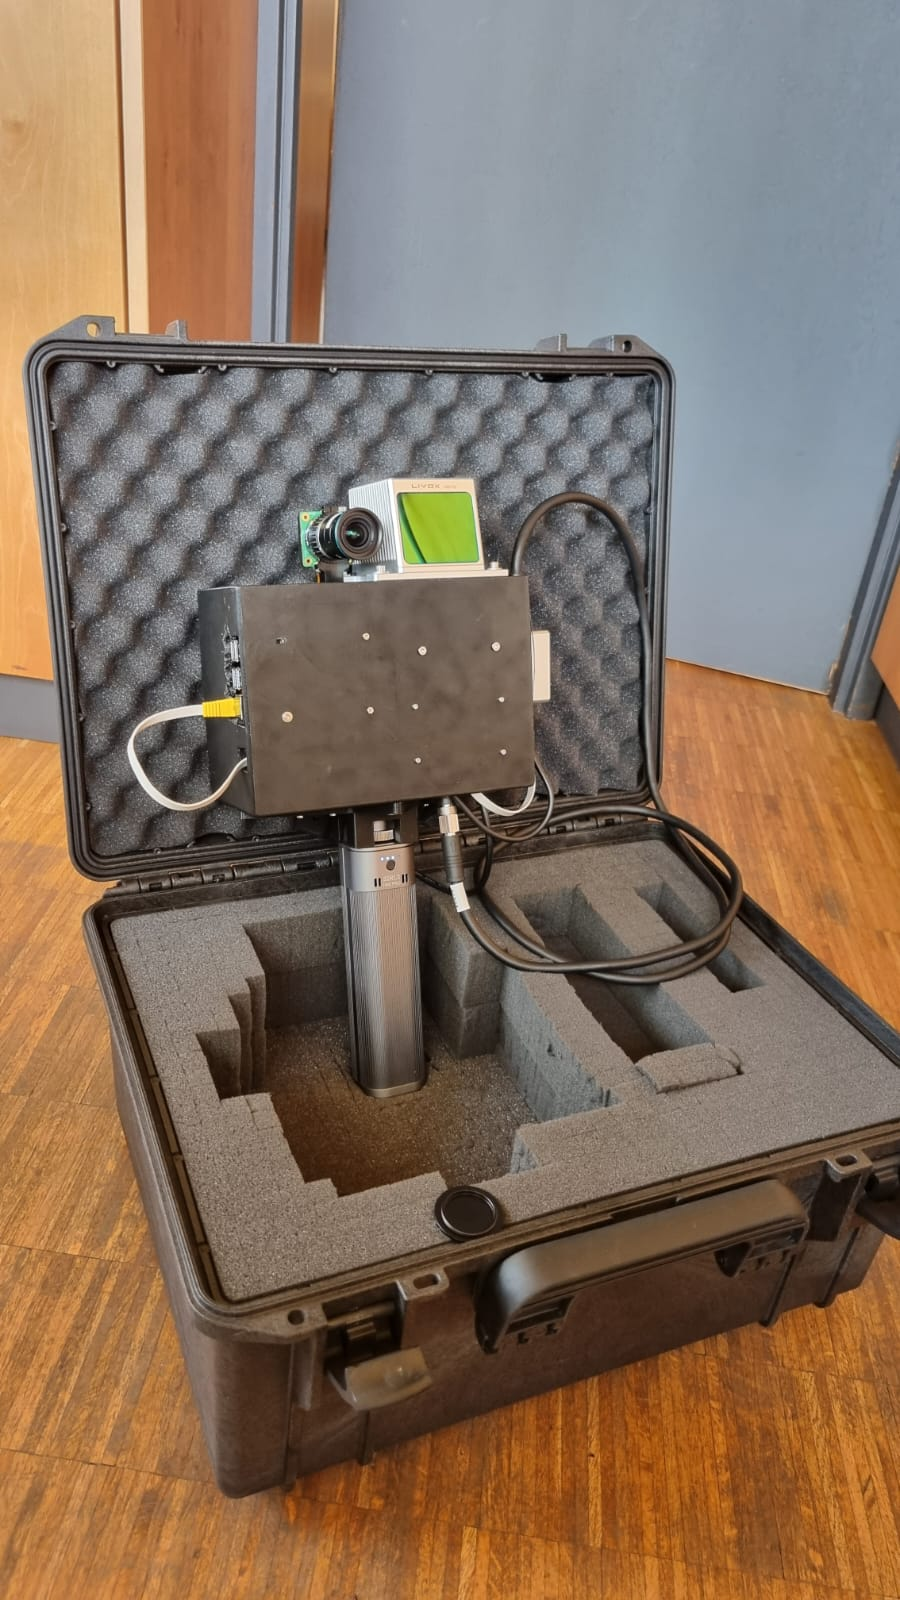
\includegraphics[width=\textwidth]{pics/handheld/WhatsApp Image 2025-09-16 at 15.05.09.jpeg}
    \end{subfigure}
    \hfill
    \begin{subfigure}[b]{0.4\textwidth}
        \centering
        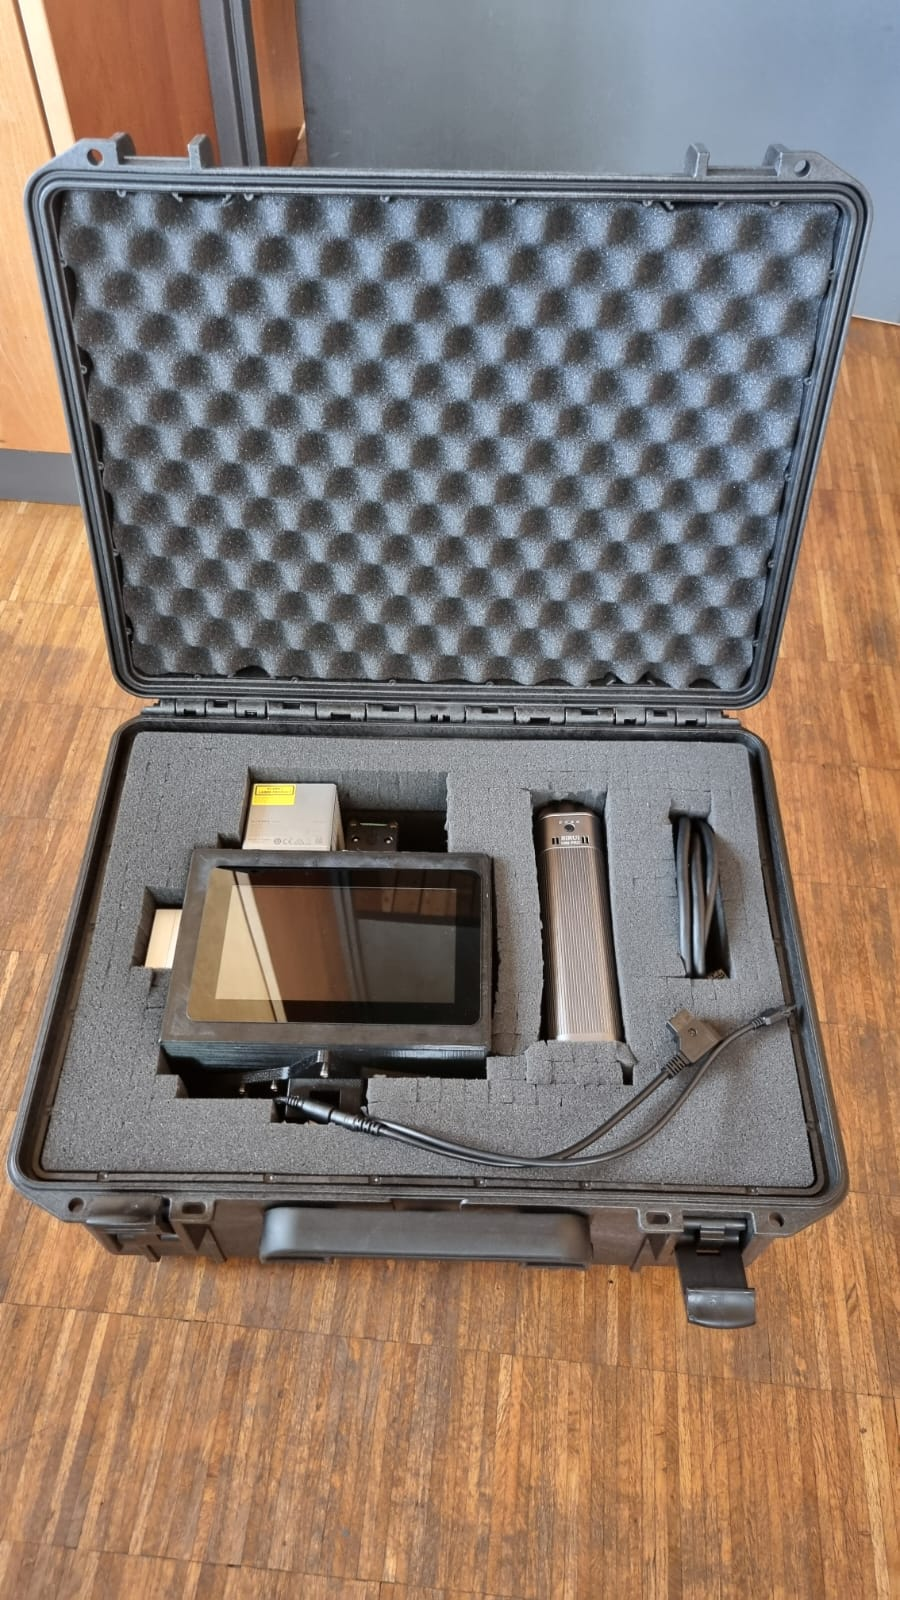
\includegraphics[width=\textwidth]{pics/handheld/WhatsApp Image 2025-09-16 at 15.05.10(1).jpeg}
    \end{subfigure}
    \caption{Pictures of handheld device}
    \label{fig:handheld_device}
\end{figure}

\begin{figure}[htbp]
    \centering
    \begin{subfigure}[b]{0.4\textwidth}
        \centering
        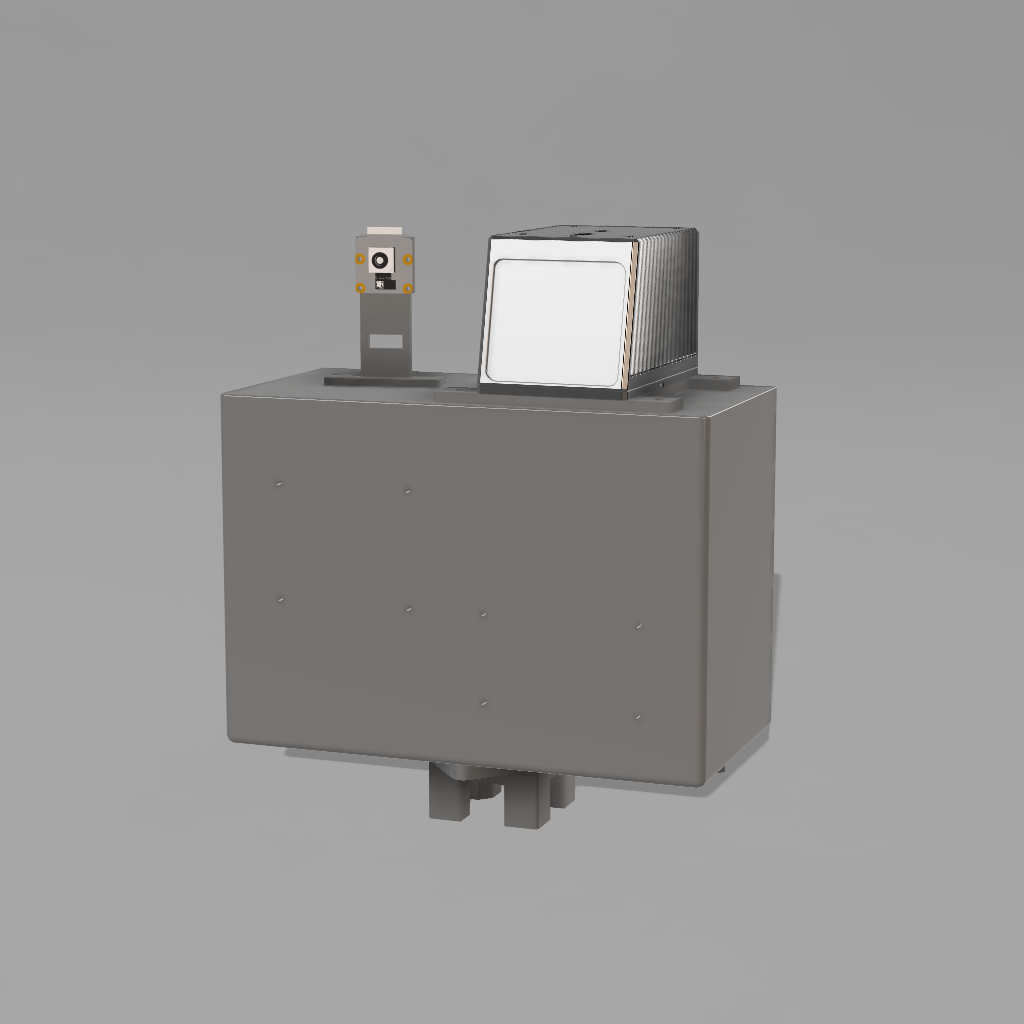
\includegraphics[width=\textwidth]{pics/Device Images/device_front_transparent.png}
        \caption{Front}
        \label{fig:bild1}
    \end{subfigure}
    \hfill
    \begin{subfigure}[b]{0.4\textwidth}
        \centering
        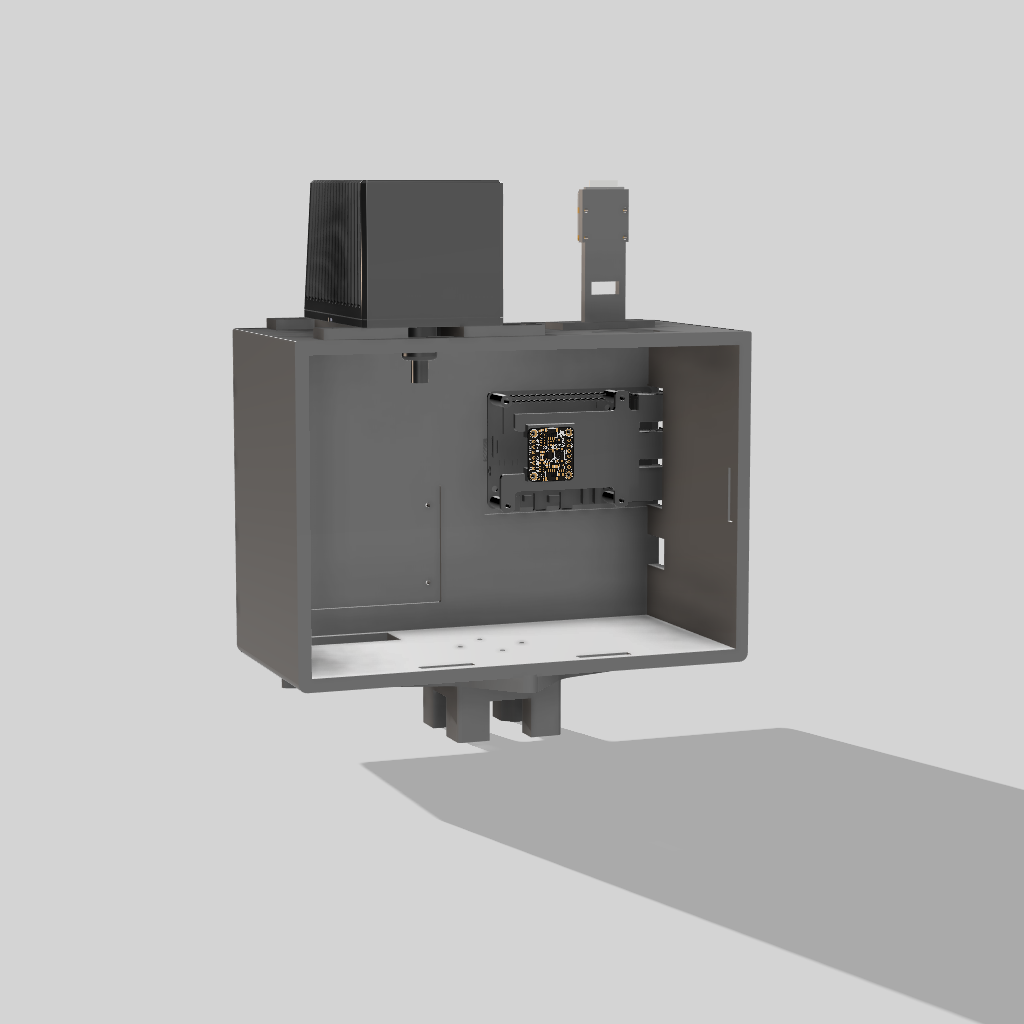
\includegraphics[width=\textwidth]{pics/Device Images/device_back.png}
        \caption{Back}
        \label{fig:bild2}
    \end{subfigure}
    \caption{Front and back of the handheld device's body}
    \label{fig:drei_bilder}
\end{figure}



\section{Components}
%\begin{figure}[htbp]
%    \centering
%    % Reihe 1
%    \begin{subfigure}[b]{0.45\textwidth}
%        \centering
%        \includegraphics[width=\textwidth]{Platzhalter.jpg}
%        \caption{PI 5}
%        \label{fig:pi5_socket}
%    \end{subfigure}
%    \hfill
%    \begin{subfigure}[b]{0.45\textwidth}
%        \centering
%        \includegraphics[width=\textwidth]{Platzhalter.jpg}
%        \caption{Mid--70}
%        \label{fig:mid_70}
%    \end{subfigure}
%    
%    \vskip 0.5cm % Abstand zwischen den Reihen
%
%    % Reihe 2
%    \begin{subfigure}[b]{0.45\textwidth}
%        \centering
%        \includegraphics[width=\textwidth]{Platzhalter.jpg}
%        \caption{BNO085}
%        \label{fig:imu_img}
%    \end{subfigure}
%    \hfill
%    \begin{subfigure}[b]{0.45\textwidth}
%        \centering
%        \includegraphics[width=\textwidth]{Platzhalter.jpg}
%        \caption{Sirui H99}
%        \label{fig:h99_sirui}
%    \end{subfigure}
%    
%    \vskip 0.5cm % Abstand zwischen den Reihen
%
%    % Reihe 3
%    \begin{subfigure}[b]{0.45\textwidth}
%        \centering
%        \includegraphics[width=\textwidth]{Platzhalter.jpg}
%        \caption{Camera Module 3}
%        \label{fig:cam_3}
%    \end{subfigure}
%    \hfill
%    \begin{subfigure}[b]{0.45\textwidth}
%        \centering
%        \includegraphics[width=\textwidth]{Platzhalter.jpg}
%        \caption{Touch Display}
%        \label{fig:touch_img}
%    \end{subfigure}
%
%    \caption{Sechs Bilder in drei Reihen und zwei Spalten}
%    \label{fig:6bilder_2spalten}
%\end{figure}

\subsection*{Raspberry Pi~5 (16GB) and M.2 Socket with SSD for Higher Speed}
The main component of the handheld device is a Raspberry Pi 5 with 16GB. 
The Raspberry Pi is an inexpensive, versatile single-board computer that, thanks to its compact design and low power consumption (5V/5A), 
can be connected directly to the Pi via a CSI interface.
However, the Raspberry Pi also has limitations: Its CPU and GPU performance is limited compared to powerful x86 systems, which can lead to 
bottlenecks in computationally intensive tasks such as real-time 3D data processing or complex AI applications. In addition, programs that 
use CUDA cannot be used, which severely limits the choice of programs for calculating depth images, for example. Despite these limitations, 
however, the Raspberry Pi offers excellent value for money and is therefore the right choice for this system, even if it means that many 
processing steps have to be outsourced to another system.
In addition, an M.2 socket is installed in combination with a solid-state drive (SSD), which expands the storage capacity and significantly 
increases the system's data transfer rates. Compared to conventional microSD cards, which often serve as the primary storage medium for the 
Raspberry Pi, M.2 SSDs offer significantly higher write and read speeds as well as improved durability. This device has a 256GB SSD installed.

\subsection*{Livox Mid-70}
    The Livox Mid-70 is a compact, cost-effective LiDAR sensor designed specifically for 3D data capture and robotics applications. 
    It offers a 70° field of view with non-repetitive scan pattern technology that enables uniform coverage of the scene and high point 
    density over time. With a range of up to 260 meters under optimal conditions and high measurement accuracy, the Mid-70 is capable of 
    generating detailed point clouds suitable for mapping, object detection, and sensor fusion. Another advantage is the compact design of the scanner. 
    However, the use of the non-repetitive scan pattern for static scenes requires a longer acquisition time to achieve complete coverage. Unlike the Livox Mid-360, 
    the Livox Mid-70 comes with an additional converter box, which makes it very easy to connect Ethernet, power supply or PPS signal cables. In addition, the 22.2V 
    from the battery can be connected directly to it without a voltage converter. However, a major disadvantage of the Mid-70 is the lack of an internal IMU, which 
    means that you have to use an external one if you want to do SLAM or similar tasks, for example. Overall, however, the Livox Mid-70 is a very good choice for 
    handheld devices like ours, as you get a solid laser scanner for the low price of around €900 as of September 2025.


\subsection*{External BNO085 IMU}
The handheld prototype employs the Adafruit BNO085, an inertial measurement unit (IMU) that combines 
a 3-axis accelerometer, gyroscope and magnetometer in a compact form factor. The BNO085 is based on 
the Bosch BNO080/BNO085 sensor and integrates a dedicated 32-bit ARM Cortex-M0+ processor running 
the \textit{Hillcrest Sensor Hub} firmware. This embedded sensor fusion engine enables real-time 
orientation estimation, providing quaternion, Euler angle, and linear acceleration outputs without 
requiring extensive host-side computation.
The device is directly connected to the PI by I\textsuperscript{2}C over the GPIO--Pins.
Due to its low power consumption, small size and ability to deliver accurate 
pose information even under dynamic motion, the BNO085 is well suited for integration into portable 
systems such as the proposed handheld LiDAR--camera device.
The choice of this sensor was also motivated by the fact that a BNO085 is integrated in the Livox 
Avia LiDAR itself.\cite{AdafruitBNO085}


\subsection*{SIRUI H99-Pro}
    When choosing a battery, we opted for the H99 Pro from SIRUI. 
    The advantage of this battery is not only that it can output up to 160W with its D-tap output (22.2V/7.5A), 
    which is more than enough for the system.
    The main reason for choosing this battery is the fact that it is a “handheld” battery and can therefore 
    be used directly as a handle.

\subsection*{Raspberry Pi Global Shutter camera}
We use the Raspberry Pi Global Shutter Camera with the Sony IMX296 sensor
(1.58\,MP, 1456$\times$1088, 3.45\,$\mu$m pixels, 1/2.9''). A 4\,mm 1/2''
C/CS-mount lens is employed; on IMX296 this yields an effective field of view
of approximately $64^\circ \times 50^\circ$ (H$\times$V) and about $76^\circ$
diagonal. The lens comfortably covers the smaller 1/2.9'' sensor, and the
global shutter exposes all pixels simultaneously.

\subsection*{Raspberry Pi Touch Display 2}
The touchscreen provides a direct interface for user interaction,  
allowing live preview, data acquisition control and system configuration.


%\subsection*{External Computer}
%\textcolor{red}{Text zu warum externer PC verwendet werden muss $\rightarrow$ Uni-Fusion}
%\begin{table}[htbp]
%\centering
%\renewcommand{\arraystretch}{1.3} % Zeilenabstand
%\begin{tabular}{>{\bfseries}l l}
%\hline
%Component & Specification \\
%\hline
%CPU (Processor) & 13th Gen Intel Core i9-13900KS x32) \\
%GPU (Graphics Card) & NVIDIA GeForce RTX 4080 16 GB GDDR6X \\
%RAM & 64,0 GB\\
%Operating System & Ubuntu 24.04 LTS\\
%\hline
%\end{tabular}
%\caption{Main PC components}
%\label{tab:pc_specs_simple}
%\end{table}

\section{Purchase costs}

Table~\ref{tab:device-costs} indicates a total hardware expenditure of approximately 1{,}327\,€,
placing the prototype squarely in the \emph{low-cost} category for 3D sensing and mapping.
While the Livox Mid70 (900\,€) constitutes the primary cost driver, the remaining components
(Raspberry~Pi~5 with accessories, camera module and optics, IMU, tripod and peripherals)
are commodity parts with comparatively modest prices. This bill of materials enables
cost-effective replication, straightforward maintenance (due to off-the-shelf availability),
and even multi-unit deployments under constrained budgets. The resulting platform is thus
well suited for teaching labs and student projects.All prices are approximate and refer to prices as of September 2025.

\begin{table}[h]
\centering
\begin{tabular}{ll}
\toprule
\textbf{device} & \textbf{$\sim$price [€]} \\
\midrule
Raspberry PI 5 (16GB)   & 130 \\
PI accessories (M2 Socket, cooler)   & 54 \\
Global Shutter camera & 60 \\
IDS 2MP objective & 100 \\
Touchpad 2 & 43 \\
Livox Mid70   & 900 \\
IMU BNO085    & 30 \\
SIRUI H99 Pro & 110 \\
other (voltage converter, cables, etc.) & 30 \\
\midrule[\heavyrulewidth] % dickere Linie für Gesamtsumme
\textbf{Overall} & \textbf{$\sim$1500} \\
\bottomrule
\end{tabular}
\caption{Listing of all device costs}
\label{tab:device-costs}
\end{table}


\chapter{Software}

The following chapter describes the structure of the software and shows which
programmes are used and gives a brief overview of the functions.
It also deals with installation problems that I myself
encountered.
The complete code files can be downloaded from the Github repository ("https://github.com/jakob2907/rasberrypi-based-LiDAR-CAMERA-rig")~\cite{github_handheld}
and tested yourself.

\section{Setup}
The handheld device presented has several sensors, including a Livox Mid 70 and
a PI camera. Since we need to process their sensor data, we use ROS 2 (Robotic Operating System), which
enables the publication and processing of data via standardised topics.
Each sensor functions as its own ROS node and can be operated independently of the others.
For this reason, instead of the Raspberry Pi's own operating system, we have installed Ubuntu 24.04.02 LTS and the
corresponding ROS 2 Jazzy, because ROS is not currently available for Raspberry Pi OS.~\cite{ros2_jazzy_releases} 

\begin{table}[h!]
\centering
\begin{tabular}{|l|l|}
\hline
\textbf{Category} & \textbf{ROS-Packages / Software} \\
\hline
LiDAR & Livox-Ros2-Driver~\cite{LivoxROS2Driver} \\
\hline
Camera & Camera-Ros~\cite{CameraROS} \\
\hline
IMU & BNO085-ROS2-Node~\cite{BNO085ROS2Node} \\
\hline
Intrinsic Calibration & own calibration script~\cite{github_handheld}\\
\hline
Extrinsic Calibration & FAST-CALIB as ROS2 package~\cite{FASTCalibROS2}\\
\hline
\end{tabular}
\caption{Overview of used ROS packages}
\label{tab:ros_packages}
\end{table}

\section{Uni-Fusion: Universal continuous mapping}

Uni-Fusion~\cite{yuan2024uni} is a universal continuous mapping framework for 3D surfaces and arbitrary sensor-derived properties, and it was
originally developed by the same research chair at which this Bachelor's thesis is being conducted. Unlike
learning-based mapping methods, Uni-Fusion does not require any pre-training, yet it can directly incorporate heterogeneous
data modalities (e.g. RGB colors, infrared intensities or even high-dimensional semantic descriptors) into a unified map
representation. This capability is achieved through a novel encoder--decoder scheme based on Gaussian
Process Regression (GPR): the approach “decouples” GPR by approximating its kernel, allowing a set of points and their
properties to be encoded as a single compact latent feature vector and later decoded to predict continuous field values. In essence, the kernel approximation (using techniques like Nyström eigenfunction decomposition)
provides a fixed position encoding function, while the local point observations are aggregated by a content encoding function
to produce a latent code. The latent code serves as the parameters of a local implicit model such that any spatial query can
be decoded (via the same kernel basis) into a predicted property value (for example, a signed distance or a color intensity) in
that region. Because this encoding--decoding model is analytic and data-agnostic, Uni-Fusion can handle
arbitrary types of point properties without specialized training or tuning for each property. The latent
representation also makes the map continuous, meaning that surface geometry and other fields are not stored on a fixed grid
but can be queried at any resolution, enabling high-fidelity outputs.

\begin{figure}[!htb]
\centering
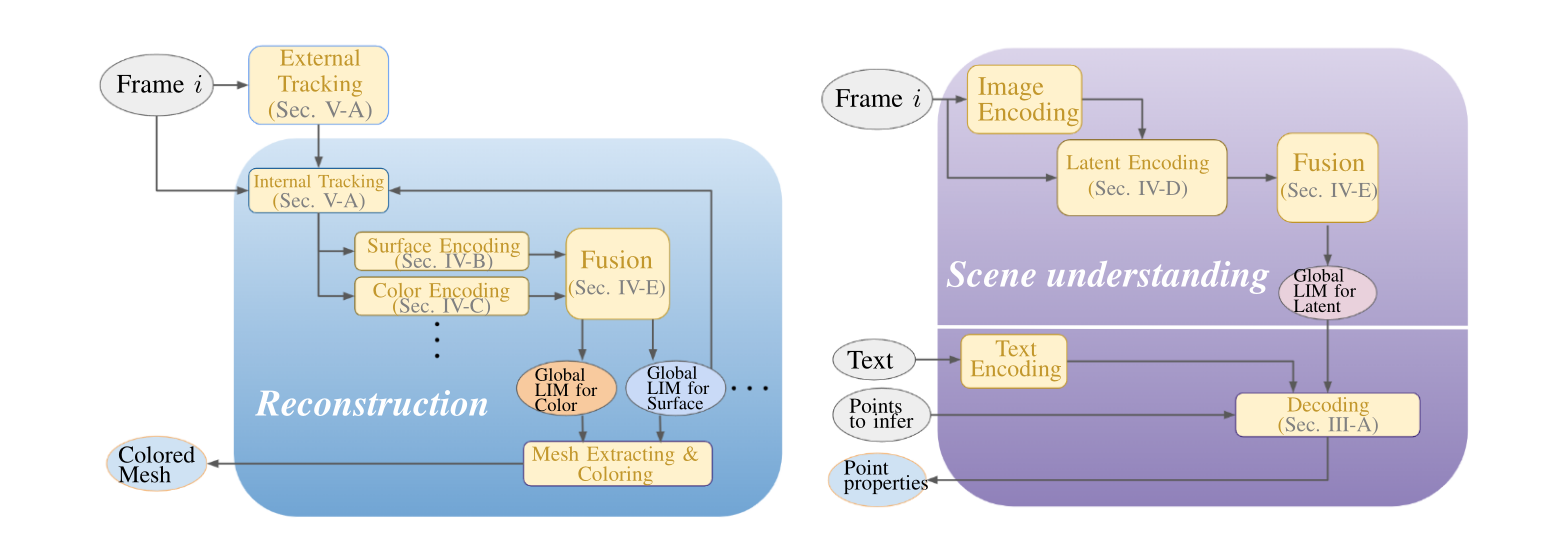
\includegraphics[width=\textwidth]{pipeline}
\caption{Overview of the Uni-Fusion mapping pipeline, which incrementally fuses per-frame latent maps into a global Latent
Implicit Map (LIM) for continuous surface and property reconstruction.\cite{yuan2024uni}}
\label{fig:pipeline}
\end{figure}
Figure~\ref{fig:pipeline} illustrates how per-frame local latent maps are fused into the global LIM.
Spatially, Uni-Fusion partitions the scene into a regular voxel grid (typically sparse in memory) and for each voxel it
aggregates local point data into a latent feature vector. This collection of latent vectors over all occupied
voxels constitutes the Latent Implicit Map (LIM) -- a continuous implicit representation of the scene's geometry and any
additional property fields. Each voxel's latent feature encodes the local geometry or other scalar/vector properties observed in
that cell, effectively acting as a locally conditioned implicit function. Incremental mapping is achieved by processing incoming
sensor frames one at a time and fusing each frame's local contributions into the global LIM. In practice, for
each new RGB-D frame (with an estimated pose from a parallel tracking system) a local LIM is computed: the depth points
(with their associated attributes) are first assigned to their respective voxels and then an encoding is performed per voxel to
update that voxel's latent feature. These local latent maps from the frame are then merged into the global latent map on a
voxel-by-voxel basis. The fusion operation can be as simple as averaging or aggregating the latent vectors using the count of
points, ensuring that the global LIM integrates information over time as more frames are observed. This design naturally supports
real-time operation: mapping is done incrementally with each frame, and the computation in each voxel is independent and
bounded by the local data, keeping the update efficient. Indeed, Uni-Fusion is reported to run as a real-time algorithm in
practice, demonstrating that the analytic latent encoding (which avoids heavy iterative optimization or neural
network inference) is fast enough for online use.

Once integrated into the global LIM, the latent representation can be converted into an explicit 3D map or other output
modalities. For example, to obtain a surface mesh, one can densely sample spatial points and decode the global latent implicit
surface (using the combined contributions of nearby voxel latents) to evaluate a continuous signed distance field; a standard
isosurface extraction (e.g. Marching Cubes) then produces a mesh of the reconstructed surface. Similarly, to render a mapped
property like color, one can query the color field at arbitrary surface points using the global color latent map, yielding a texture
or per-vertex coloring for the mesh. Because the latent map encodes a continuous field, these queries can be made at arbitrarily
fine resolution, which means the reconstruction is not limited by voxel size in detail. Crucially, Uni-Fusion's framework supports
multi-modal mapping concurrently: for instance, in an RGB-D reconstruction scenario, two LIMs are maintained in parallel -- one
for geometry (surface occupancy or SDF) and one for color -- and both are updated with each frame. The system's design cleanly
generalizes beyond RGB-D data; additional data channels (such as infrared readings or learned feature vectors)
can be handled by simply introducing additional PropertyMap instances that use the same
GPR-based encoder on the new data type. No retraining or architectural change is needed to incorporate a
new property -- the kernel-based encoder will compute latent codes for the new values just as it does for color, given raw input
pairs of 3D coordinates and property values. Impressively, the authors demonstrate even a high-dimensional CLIP embedding
field: image features from a pre-trained vision-language model are projected onto the surface, and Uni-Fusion builds a LIM that
stores, for each region of the scene, a latent feature encoding the local CLIP descriptors; this allows semantic queries (in the
form of text prompts) to be answered by comparing the stored CLIP features to text embeddings, effectively achieving open-
vocabulary semantic mapping on the 3D surface. The flexibility to handle such diverse inputs in one mapping
system underscores the “universal” nature of Uni-Fusion.

In summary, Uni-Fusion enables real-time, incremental 3D mapping that unifies geometry and semantics in a single continuous
representation. The method's key insight is to use a decoupled GPR encoder -- decoder to directly produce local implicit functions
(Latent Implicit Map cells) from raw sensor data, avoiding any network training and associated runtime costs. As new data arrives,
the latent map is refined on-the-fly by fusing local latent updates, resulting in a globally
consistent scene representation that can be queried for detailed surfaces or property values at will. The fact that this Bachelor's
thesis is conducted within the same institute that developed Uni-Fusion has provided a unique opportunity to build upon and
closely examine this cutting-edge mapping framework.

\chapter{Approach}
\label{sec:approach}

In this chapter, the methodological approach of the work is introduced. The goal is to
outline the sequence of steps (shown in \ref{fig:schematic_workflow}) taken to achieve the intended results. Starting with the
acquisition of raw data, the subsequent stages of preprocessing, processing and evaluation
are presented. Each step is described to provide a transparent overview of the applied
procedure and to ensure reproducibility of the approach.

\begin{figure}[ht!]
    \centering
    %pipeline_diagram.png
    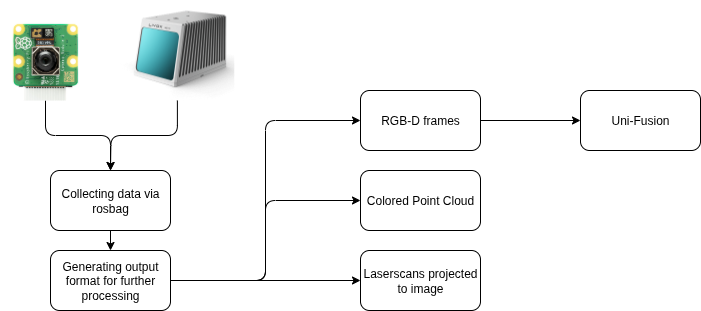
\includegraphics[width=\linewidth]{pics/Approach.png}
    \caption{Schematic representation of the data processing chain}
    \label{fig:schematic_workflow}
\end{figure}

\section*{Gathering data from device}
The initial step of the approach involves the systematic acquisition of raw data from the
developed device. For this purpose, three complementary sensors are integrated: a Livox
Mid-70 LiDAR scanner, a BNO085 inertial measurement unit (IMU) and a Raspberry PI Global Shutter camera.
Each of these components contributes essential information required for subsequent data
processing. The Livox Mid-70 provides dense three-dimensional point clouds that describe
the spatial structure of the environment. The BNO085 IMU delivers inertial data, including
acceleration and rotational velocity, since the IMU is essential for obtaining reliable
pose estimates while the device is in motion and for enabling future applications such as SLAM.
In addition, the Global shutter camera captures image sequences that offer visual context
and enable to color pointclouds. To ensure synchronized and reproducible data collection, the
Robot Operating System (ROS) framework is employed. All sensor streams are recorded using
the rosbag tool, which stores the data in a structured format that preserves
timestamps and message integrity. This unified recording approach enables consistent
alignment of heterogeneous data sources and provides a reliable basis for subsequent
preprocessing, calibration and evaluation steps.

\section*{Generating output for further processing}

After the raw data has been recorded using rosbag, we create a hierarchical folder structure so 
that we can export the data. Theoretically, the depth images and other data could also be generated on 
the Raspberry PI. However, since its performance is very limited and you will need to switch to a more 
powerful device later on due to the performance required for Uni Fusion, we can also process the data on 
this higher performing device. On top of that the usage of the other device also enables us to use
CUDA-based programs, like Open3D.

The output folder contains a {index.txt} file. This file serves as a mapping between each scan folder
and its corresponding underlying ROS bag file. Furthermore, the folder contains a JSON file that provides
the recorded IMU measurements together with their corresponding timestamps, ensuring an explicit temporal association of the data.
In addition, a separate scan\_xx folder is created for each registered scan that we receive via 
the livox topic (/livox/lidar), with the identifier at the end being incremented 
chronologically. Each scan folder contains the points of the recorded point cloud once as a numpy array 
(.npy) and as a .pts file. In addition, the associated image (.png) and the 
timestamp (.txt) of when the scan was recorded by PointCloud and Image are saved.
When creating the scanfolder we check if the timestamp between the Livox scan and the captured image
is close to each other. This ensures that a scan is not matched with an image recorded at a substantially
different time; in our case, temporal alignment is defined as a maximum acquisition time difference of 10 ms.
The synchronization of the sensors and the use of a common time standard are ensured via the Precision Time 
Protocol (PTP), see~\ref{sec:PTP}.

\begin{figure}[ht!]
    \begin{verbatim}
    \output_dir{
        imu_data_(name of rosbag).json
        index.txt
        scan_001/
            pointcloud.npy
            pointcloud.pcl
            image.png
            timestamp.txt
        scan_002/
            ...
    }
\end{verbatim}
\end{figure}

\section*{Data processing}
This work presents three data-processing pathways. First, depth images are generated from
LiDAR and camera data and used to compose RGB-D input frames for Uni-Fusion. Second, a
routine produces colored point clouds from multiple frames to assess the extrinsic
calibration between the LiDAR and the camera. Third, the same routine supports the
``opposite direction,'' i.e., projecting LiDAR point-cloud points into the image domain.

\subsection*{Depth-Images for RGB-D}
In order to prepare the data for subsequent RGB-D fusion, a dedicated generation process was 
implemented. The goal is to produce pairs of RGB frames and corresponding depth images that are 
aligned and can be directly consumed by fusion frameworks such as Uni -- Fusion. Each scan 
directory contains a synchronized LiDAR point cloud and an RGB image. Using the known extrinsic 
and intrinsic calibration parameters, the LiDAR points are projected into the camera coordinate 
system. Based on this projection, a depth map is constructed in which each pixel encodes the 
distance of the nearest LiDAR point to the camera. Empty pixels remain black at first, while valid pixels 
are normalized to an 8-bit intensity representation to ensure compatibility with standard image 
formats.
Together with the original RGB frame, these depth maps are stored in a structured output 
folder, where each frame is saved as frameXXX.png and the corresponding depth map as 
depthXXX.png. This systematic naming convention ensures that both modalities remain 
synchronized across all frames of a scan sequence. By organizing the data in this format, the 
pipeline produces ready-to-use input that enables efficient integration into RGB-D based Uni--Fusion
and supports reproducibility of experiments.

\begin{figure}[ht!]
    \begin{verbatim}
    \output_dir{
        cam_params.json 
        depth001.png
        depth002.png
        depth...
        frame001.png
        frame002.png
        frame...
        (mesh.ply)
    }
\end{verbatim}
\end{figure}

\subsection*{Sparse Depth Image}
\label{sec:sparsedepth}
The Livox Avia LiDAR provides less than 10,000 points per individual scan.
While this number may be sufficient for certain tasks such as simple mapping or coarse object detection, 
it is very limited when compared to the requirements of dense depth image generation. 
A depth image with a resolution of $640 \times 480$ pixels contains a total of 307,200 pixels.
If only 10,000 points are projected into this image space, approximately one out of 31 pixels,
that is around $3.25\%$, will actually receive a depth value.
In combination with its flower -- shaped scanning pattern
the resulting image is therefore extremely sparse, and large portions of the image remain undefined (see Figure \ref{fig:sparse_depth}). 
This low density is not adequate for applications that rely on detailed depth maps.

\begin{figure}[ht!]
    \centering
    %pipeline_diagram.png
    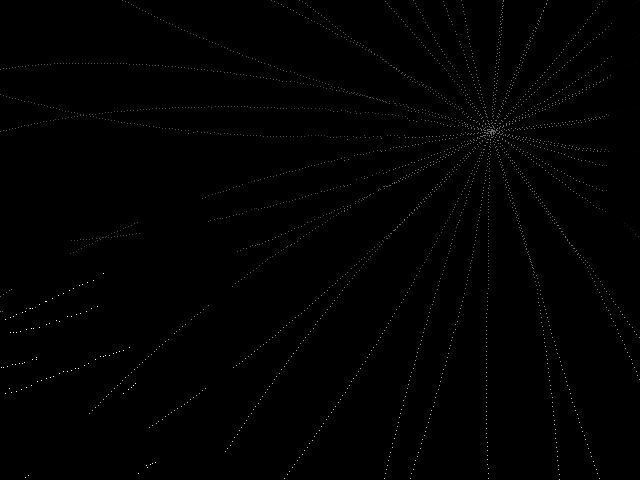
\includegraphics[width=\linewidth]{pics/depth_no_icp_robohall.png}
    \caption{Sparse Depth Image}
    \label{fig:sparse_depth}
\end{figure}

\begin{figure}[ht!]
    \centering
    %pipeline_diagram.png
    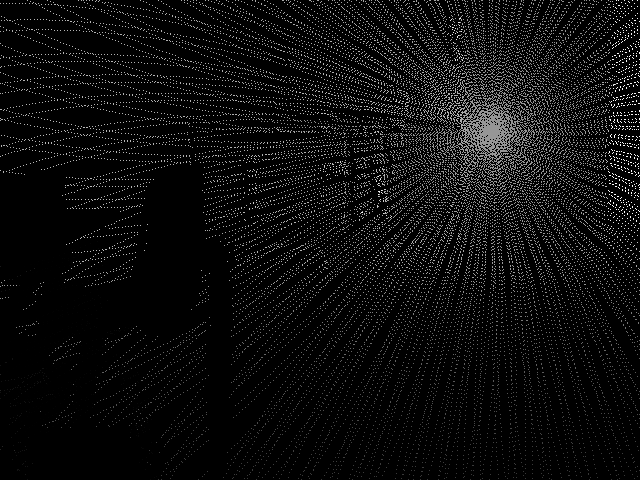
\includegraphics[width=\linewidth]{pics/depth_icp_robohall.png}
    \caption{Depth Image with ICP Alignment of several scans}
    \label{fig:icp_depth}
\end{figure}

\begin{figure}[ht!]
    \centering
    %pipeline_diagram.png
    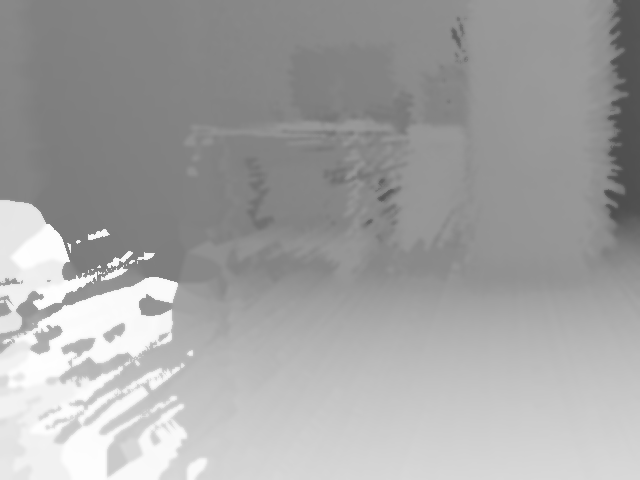
\includegraphics[width=\linewidth]{pics/depth_filled_robohall.png}
    \caption{Depth Image with ICP and bilinear Interpolation}
    \label{fig:icp_filled_depth}
\end{figure}

In this implementation, sparsity is mitigated in a purely geometric manner. Rather than relying solely on the
most recent LiDAR frame, consecutive scans are accumulated into a global point cloud via scan-to-map registration
using the Iterative Closest Point (ICP) algorithm. Each incoming scan is aligned to the growing map, so the set
of points projected into the camera frame includes valid measurements from previously acquired scans. This
accumulation markedly increases the number of points that project onto the image plane, thereby improving the
effective coverage in the $640 \times 480$ depth images (see Figure~\ref{fig:icp_depth}).
After projection, gaps remain because not every image location receives a measurement, even with multiple
aligned scans. To address this, a bilinear interpolation scheme assigns plausible depth values to undefined
pixels. This step smooths the depth map and yields a visually more complete representation of the scene (see
Figure~\ref{fig:icp_filled_depth}), although the accuracy remains limited compared to advanced learning-based
completion methods.
A further limitation of this incremental mapping strategy is the warm-up required for the global map to
accumulate sufficient points for adequate image-plane coverage. Consequently, the first few scans—containing
relatively few points—produce depth images with very low density.

In contrast to this straightforward interpolation and alignment strategy, Bleier et al.\ address the problem
of sparse depth images with a learning-based completion method. Their approach, named ScaleCov
~\cite{bleier2024}, builds upon the earlier DepthCov concept (Dexheimer and Davison, 2023~\cite{dexheimer2023learning}) by introducing 
a learned covariance function as a prior for depth estimation. Instead of directly regressing the full depth 
map from sparse LiDAR input --- which often leads to unreliable predictions in regions without true depth 
measurements --- ScaleCov integrates monocular depth estimates from Metric3Dv2 as an additional source 
of information. Using the available LiDAR returns, the method computes scale adjustments for pixels 
where valid depth is observed and propagates this information across the image. This strategy results in 
significantly denser and more accurate depth maps compared to simple interpolation, and it also produces 
a depth variance map that highlights areas of high uncertainty such as the sky or unobserved surfaces. 
These confidence estimates enable a more reliable integration of the completed depth data into downstream 
tasks like semantic mapping or 3D scene reconstruction.


\subsection*{Colored PointCloud}
In addition to the generation of RGB-D frames, the pipeline also supports the creation of colored 
pointclouds. While depth images encode only the geometric distance information of the scene, 
colored pointclouds enrich the LiDAR data with appearance information from the RGB images. The 
process begins by projecting all LiDAR points into the image space using the intrinsic and extrinsic 
calibration parameters. The underlying mathematics of this projection has already been introduced in 
the section \ref{sec:proj_lidar_image}, where the transformation from 3D LiDAR 
coordinates into 2D image coordinates is described in detail. Based on this mapping, only those 
points are considered that are visible within the field of view of the camera, thereby discarding 
all points that lie behind the camera plane or outside the image boundaries. For every visible 
point, the corresponding pixel in the RGB frame is identified and its color value is assigned to 
the 3D coordinate. As a result, the output is a pointcloud in which each entry consists of six 
values, representing the 3D position $(x, y, z)$ together with the associated color components 
$(r, g, b)$. The generated colored pointclouds are not only useful for visualization but also serve 
as valuable input for further reconstruction and semantic mapping tasks, since they combine precise 
geometric information with rich appearance cues from the environment.

\subsection*{Projection of pointcloud to image}
Besides generating colored pointclouds, the reverse operation, namely projecting the pointcloud 
back into the image space, was also performed. This functionality serves as a simple yet effective 
diagnostic tool to verify whether the LiDAR sensor and the camera share overlapping fields of view. 
By transforming the LiDAR points into the coordinate system of the camera and then mapping them 
onto the image plane, one can directly visualize which regions of the captured frame are covered by 
LiDAR measurements. If the projected points uniformly fill the image space, it indicates that the 
scanning range of the LiDAR aligns well with the camera's perspective, ensuring that both sensors 
observe the same part of the environment. Conversely, visible gaps or incomplete coverage in the 
projection would reveal calibration errors or misalignment in the sensor setup. This reverse 
projection therefore provides a straightforward method to assess the spatial consistency of the 
recordings and guarantees that the generated RGB-D data can later be reliably fused. The underlying 
mathematical transformations correspond to those described in the section \ref{sec:proj_lidar_image},
applied in the inverse direction for the specific purpose of coverage validation.

\section*{RGB-D frames in Uni-Fusion}  
The generated RGB-D output is directly compatible with the input requirements of Uni--Fusion. Each 
scan sequence produces a structured set of paired RGB frames and depth images that are named in a 
consistent format (frameXXX.png and depthXXX.png). This naming scheme ensures 
that the temporal correspondence between both modalities is preserved across all frames. Uni--Fusion 
expects such synchronized image pairs to be specified in a configuration file, where the dataset is 
defined using a yaml description. Within this file, the paths to the RGB and depth image 
directories are listed, together with the corresponding calibration parameters, so that Uni--Fusion 
can correctly interpret the metric depth values during reconstruction. Since the output generated 
by the pipeline already follows the required structure, the integration into Uni--Fusion is seamless. 
This design choice not only reduces preprocessing overhead, but also guarantees that the data can be 
immediately used for volumetric fusion and scene reconstruction, making the generated RGB-D frames 
a central component in the overall workflow.

\chapter{Experiments and results}
\label{sec:experiments}
\section{RGB-D}

To generate depth images from the data recorded with the laser scanner, different approaches were investigated, 
which differ in their methodological setup and in the requirements for preprocessing and data fusion. The following 
subsections describe two main strategies: single static capture and multiple static captures requiring ICP 
registration.

\subsubsection*{Single Static Capture}
In the case of a single static capture, the process is comparatively simple, since each point cloud can be processed 
independently without explicit registration with further scans. This allows a direct projection of the three-
dimensional point data onto the image plane, resulting in depth information represented as grayscale or color images. 
For this approach, the camera position in relation to the point cloud is particularly important, as only then a 
consistent depth representation can be ensured. The result is a straightforward and computationally efficient 
workflow for generating depth images from individual scans.

\subsubsection*{Multiple Static Captures with ICP}
If more than one static scan is taken, the different point clouds must be aligned with each other in order to obtain 
a consistent reconstruction of the scene. For this purpose, registration methods such as the Iterative Closest Point 
(ICP) algorithm are required, which compute an accurate overlap of the scans by minimizing point distances. By fusing 
several scans, a denser point cloud model is obtained, which significantly increases the quality of the generated 
depth images but is associated with additional computational cost.

%\subsubsection*{Dynamic Captures with SLAM}
%The case of dynamic recordings is more complex, where the sensor is continuously moved. In this scenario, SLAM 
%methods (Simultaneous Localization and Mapping) are necessary, since not only the point clouds must be registered 
%but also the sensor trajectory has to be estimated simultaneously. The calibration and integration of the Inertial 
%Measurement Unit (IMU) play a central role here, since only through the fusion of visual and inertial measurements a 
%robust and consistent reconstruction can be achieved. The resulting depth images from this approach are able to 
%represent larger and more complex environments in high resolution and with high geometric consistency, which is 
%particularly relevant for applications in mobile robotics or augmented reality.


\subsection{Experiment 1}

This experiment is based on a single static scan captured in the KUKA Lab. As illustrated in
Figure~\ref{fig:rgb_sparse}, the left panel (a) shows the original RGB image, while the right panel (b)
shows the corresponding colored point cloud. The color information is mapped from the RGB image onto the
reconstructed 3D geometry, enabling an intuitive visual linkage between 2D appearance and 3D structure.

To assess scan-to-map registration, we compare two ICP variants using depth images (see
Figure~\ref{fig:interp_completed}): ICP on the raw depth image (Figure~\ref{fig:interp_completed}, panel
(c)) and ICP on a bilinearly interpolated depth image (Figure~\ref{fig:interp_completed}, panel (d)).

Qualitatively, the bilinear interpolation reduces quantization and staircase artifacts in the depth field,
yielding smoother correspondences, more stable ICP convergence, and fewer local misalignments, especially
along slanted surfaces and at geometric edges. A minor trade-off is a slight smoothing of very fine
structures, which can attenuate subtle details.

Conclusion: In this static scan setting, the interpolated-depth variant produces a crisper alignment and a
more visually coherent geometry compared to the raw-depth ICP baseline, while preserving the essential
structure of the scene observed in Figure~\ref{fig:rgb_sparse}.

\begin{figure}[H]
  \centering
  \begin{minipage}{0.48\textwidth}
    \centering
    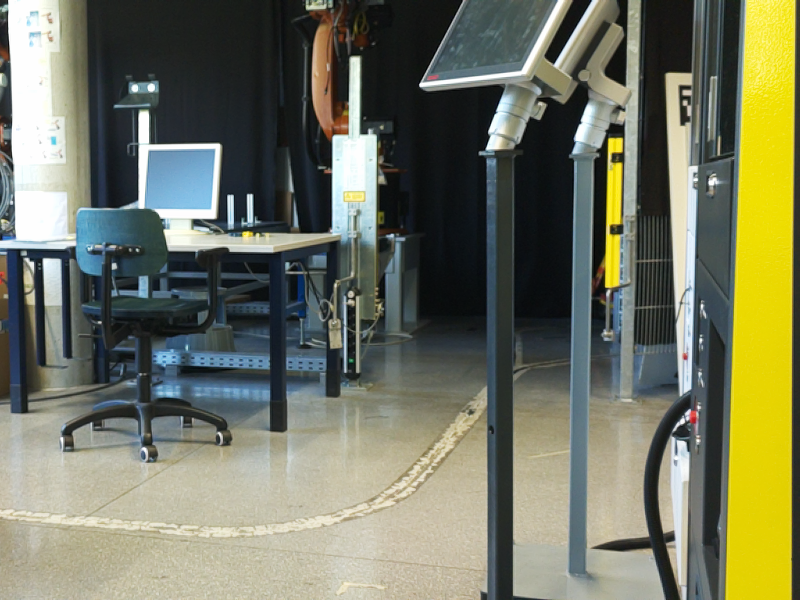
\includegraphics[width=\linewidth]{pics/KUKA_LAB_RGB.png}
    \caption*{(a) Original RGB image}
    \label{fig:col_pcl}
  \end{minipage}\hfill
  \begin{minipage}{0.48\textwidth}
    \centering
    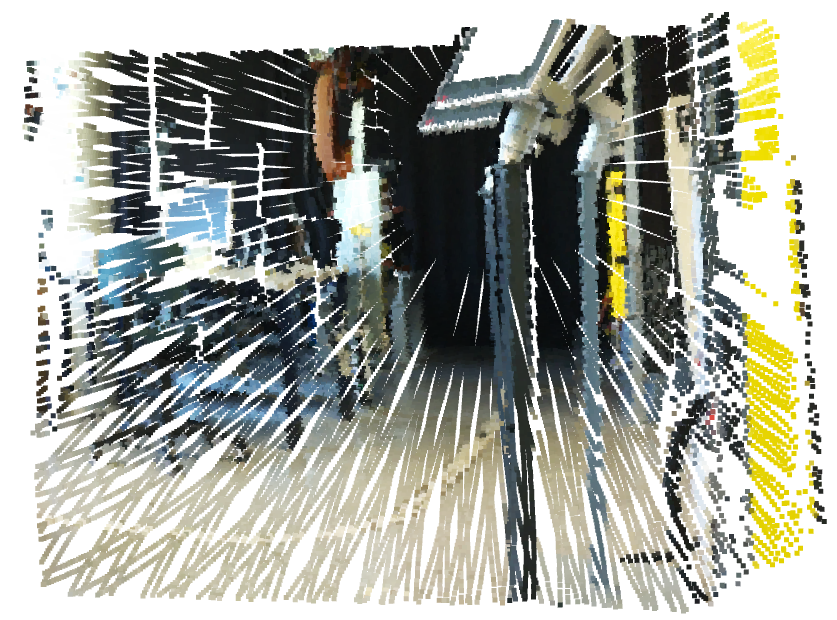
\includegraphics[width=\linewidth]{pics/KUKA_Lab_colored_plc.png}
    \caption*{(b) Colored PointCloud}
  \end{minipage}
  \caption{Example of an RGB image and the corresponding colored pointcloud.}
  \label{fig:rgb_sparse}
\end{figure}

\begin{figure}[H]
  \centering
  \begin{minipage}{0.48\textwidth}
    \centering
    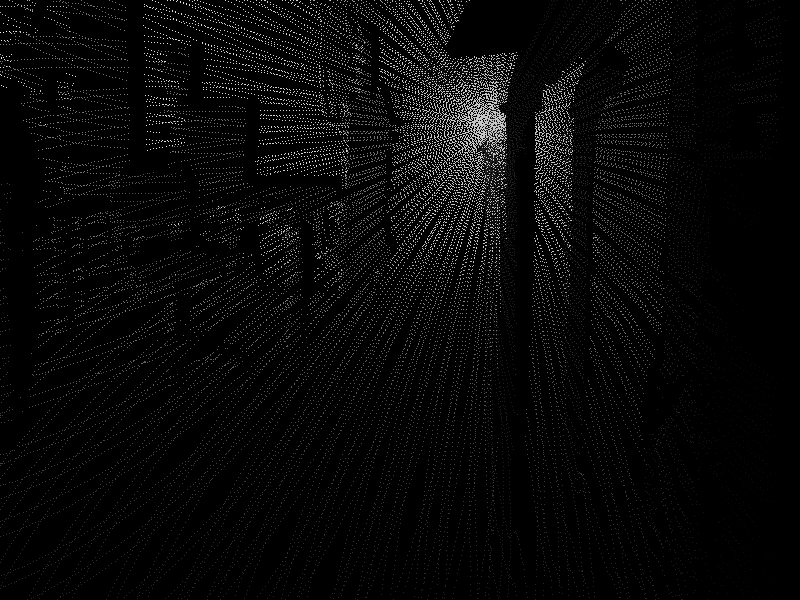
\includegraphics[width=\linewidth]{pics/KUKA_Lab_Depth.png}
    \caption*{(c) ICP aligned image}
  \end{minipage}\hfill
  \begin{minipage}{0.48\textwidth}
    \centering
    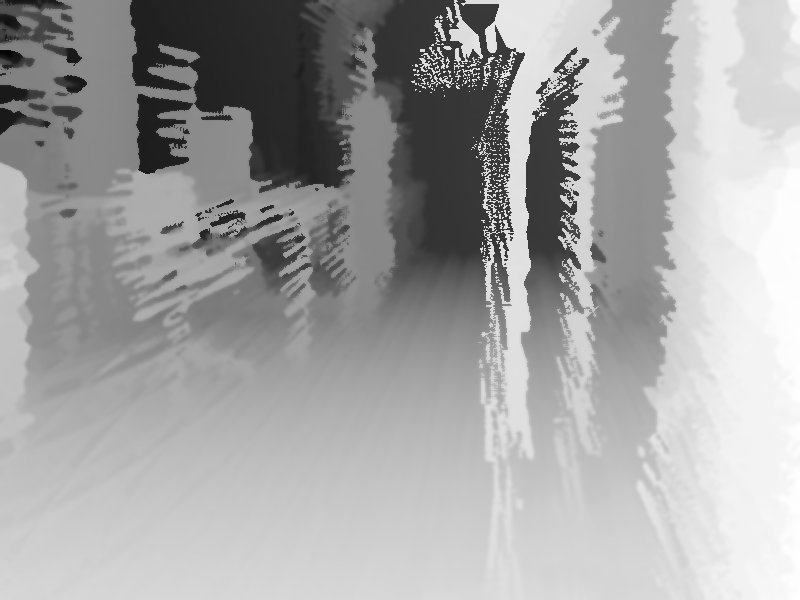
\includegraphics[width=\linewidth]{pics/KUKA_filled.png}
    \caption*{(d) ICP + bilinear interpolation depth image}
  \end{minipage}
  \caption{}
  \label{fig:interp_completed}
\end{figure}

\subsection{Experiment 2}

Experiment 2 consists of four single static scans captured in the robotics hall. Each column corresponds to a
distinct viewpoint (robo\_1 to robo\_4). The first row shows RGB frames, the second row shows depth images
aligned to the map via ICP, the third row shows the corresponding raw depth inputs, and the fourth row presents
visualization snapshots of the registered reconstructions. This layout allows a side-by-side comparison across
viewpoints and modalities, highlighting how ICP alignment improves geometric consistency relative to the raw
depth while preserving the scene structure visible in the RGB images.

\begin{table}[h]
\centering
\begin{tabular}{
  >{\centering\arraybackslash}m{0.22\textwidth}
  >{\centering\arraybackslash}m{0.22\textwidth}
  >{\centering\arraybackslash}m{0.22\textwidth}
  >{\centering\arraybackslash}m{0.22\textwidth}
}
    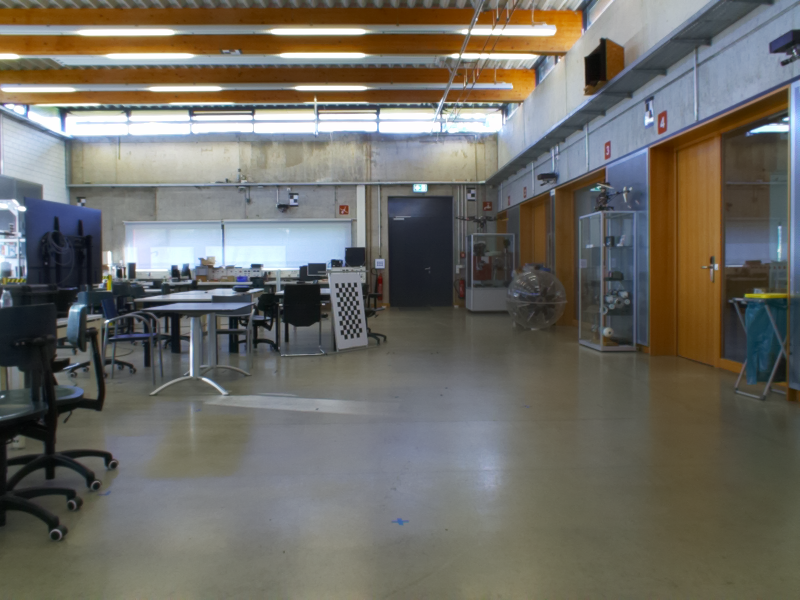
\includegraphics[width=\linewidth]{pics/robo/robo_1/image.png} &
    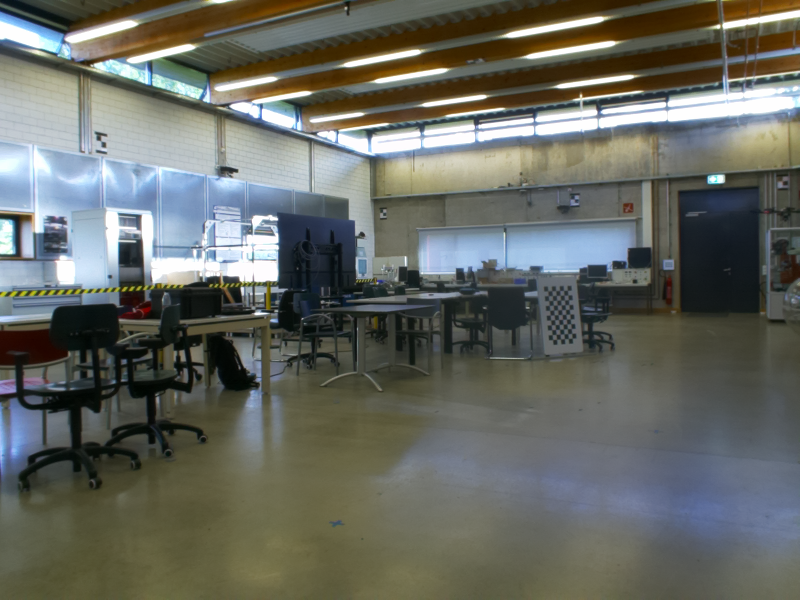
\includegraphics[width=\linewidth]{pics/robo/robo_2/image.png} &
    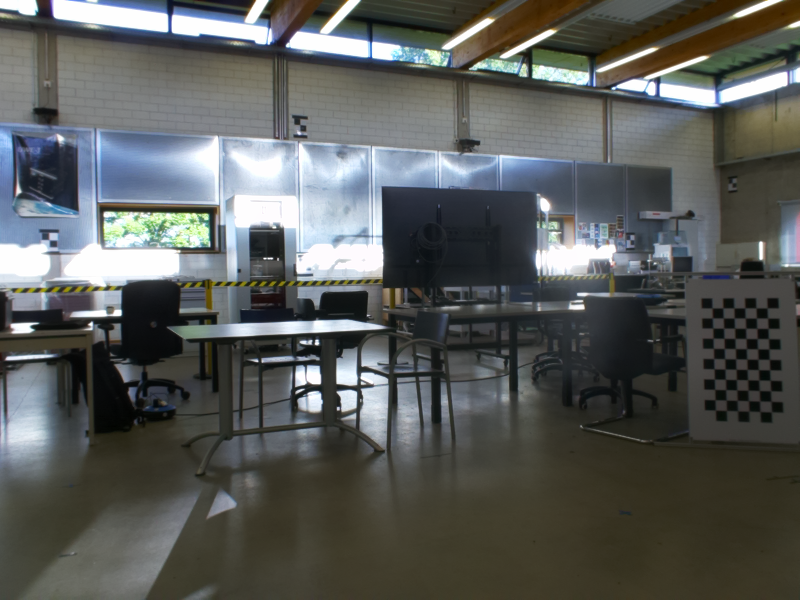
\includegraphics[width=\linewidth]{pics/robo/robo_3/image.png} &
    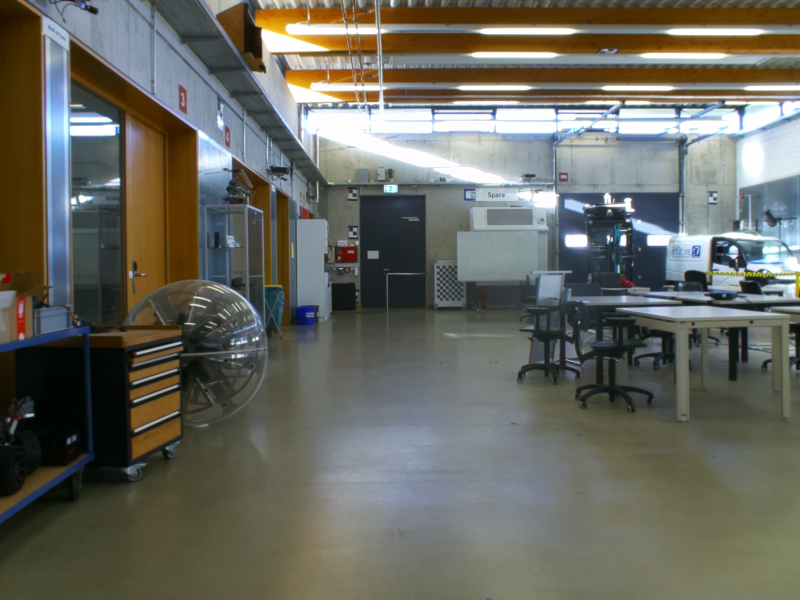
\includegraphics[width=\linewidth]{pics/robo/robo_4/image.png} \\
    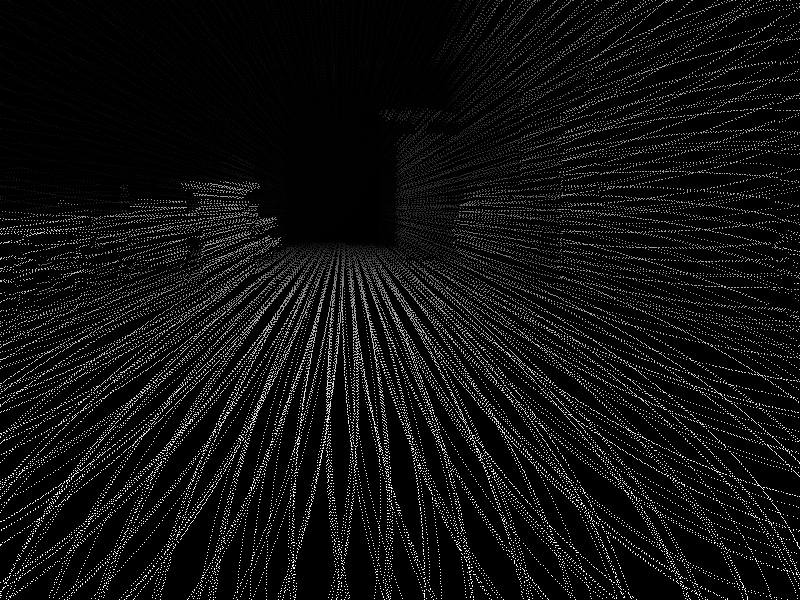
\includegraphics[width=\linewidth]{pics/robo/robo_1/depth0016_aligned.png} &
    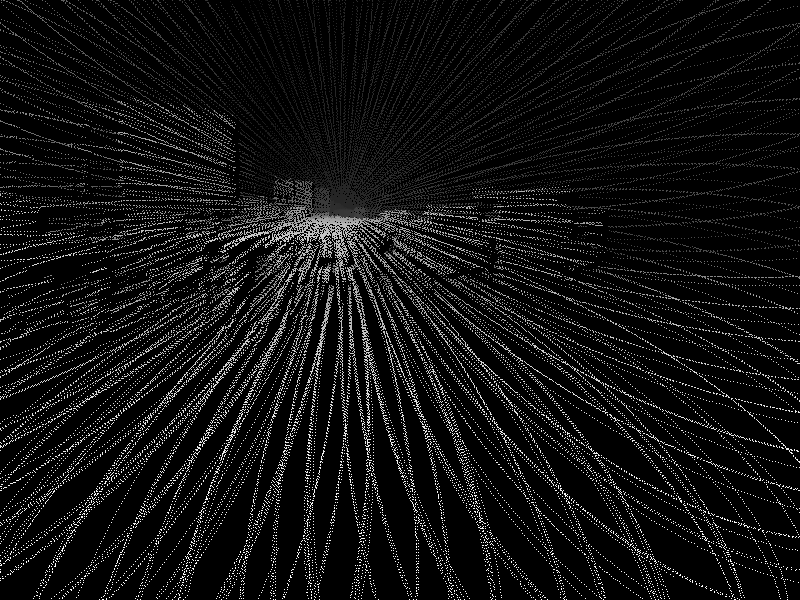
\includegraphics[width=\linewidth]{pics/robo/robo_2/depth0016_aligned.png} &
    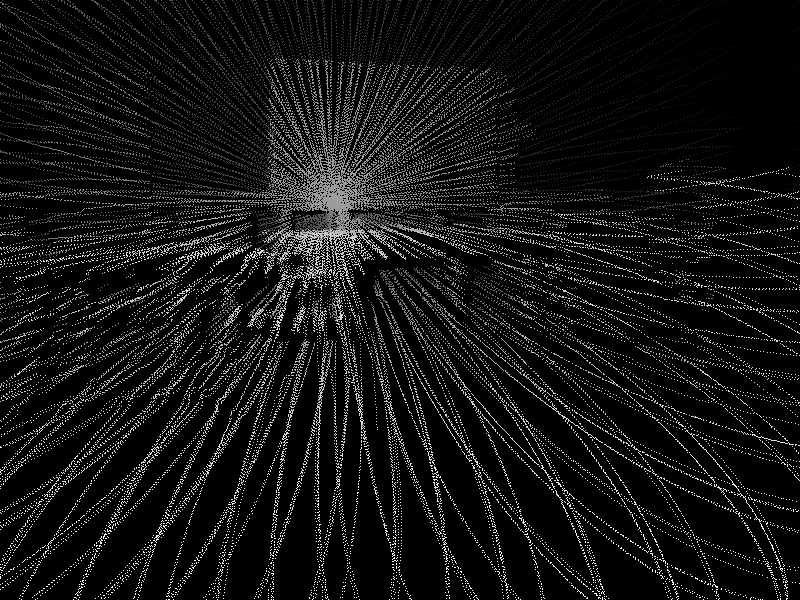
\includegraphics[width=\linewidth]{pics/robo/robo_3/depth0016_aligned.png} &
    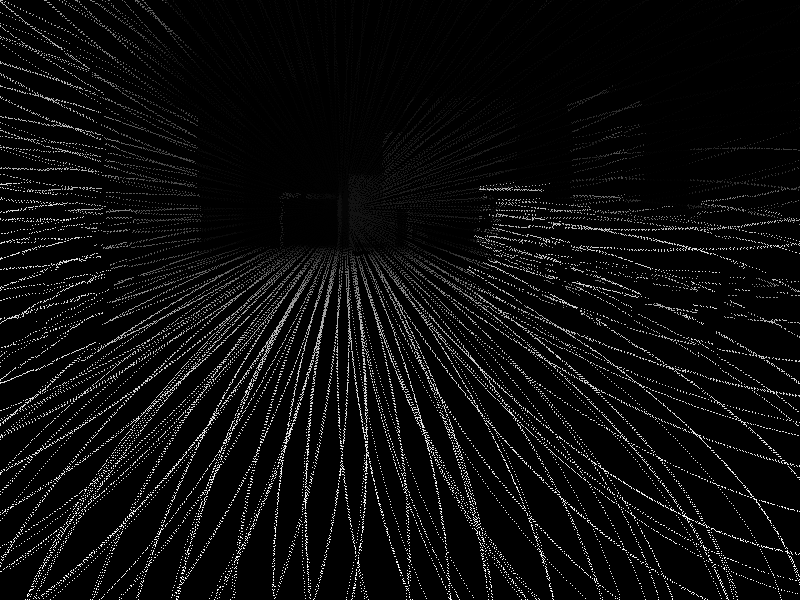
\includegraphics[width=\linewidth]{pics/robo/robo_4/depth0016_aligned.png} \\
    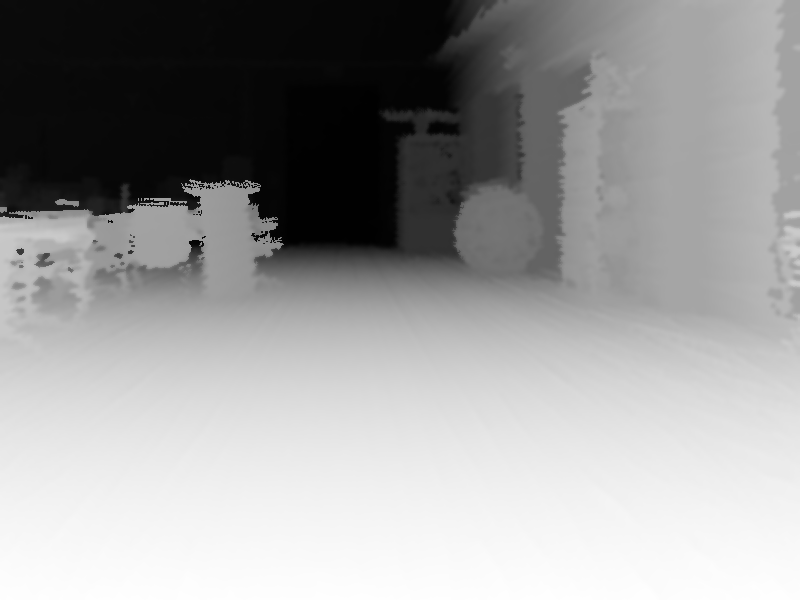
\includegraphics[width=\linewidth]{pics/robo/robo_1/depth0016.png} &
    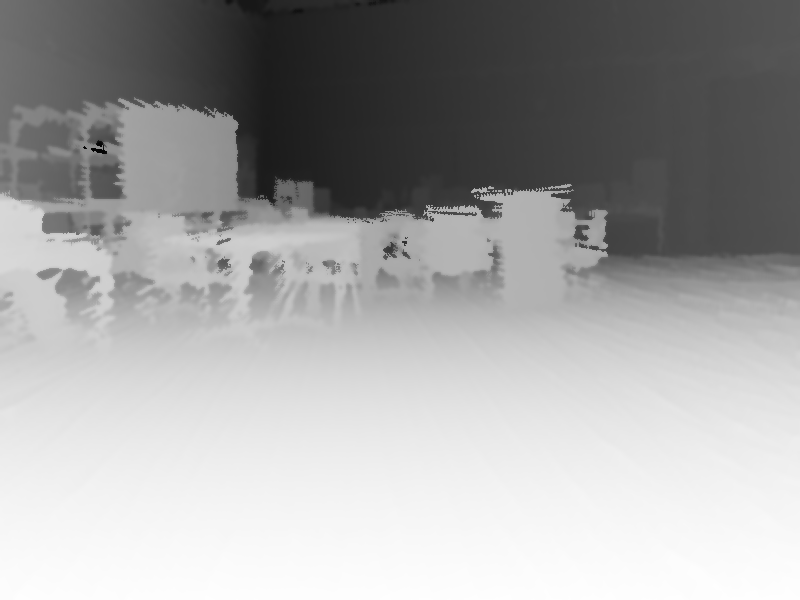
\includegraphics[width=\linewidth]{pics/robo/robo_2/depth0016.png} &
    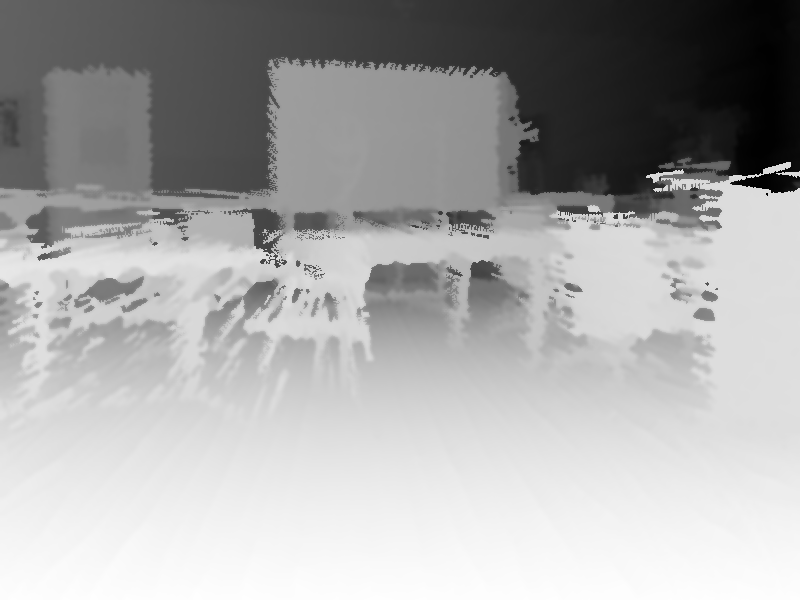
\includegraphics[width=\linewidth]{pics/robo/robo_3/depth0016.png} &
    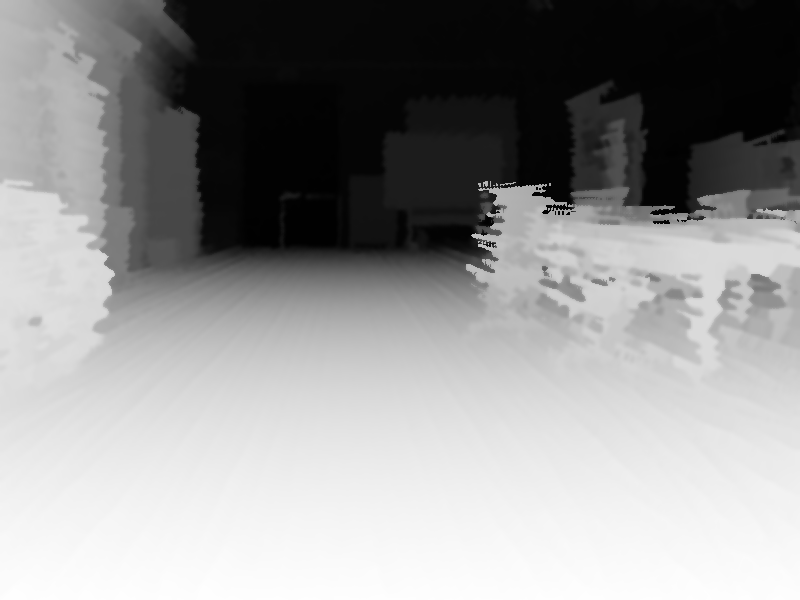
\includegraphics[width=\linewidth]{pics/robo/robo_4/depth0016.png} \\
    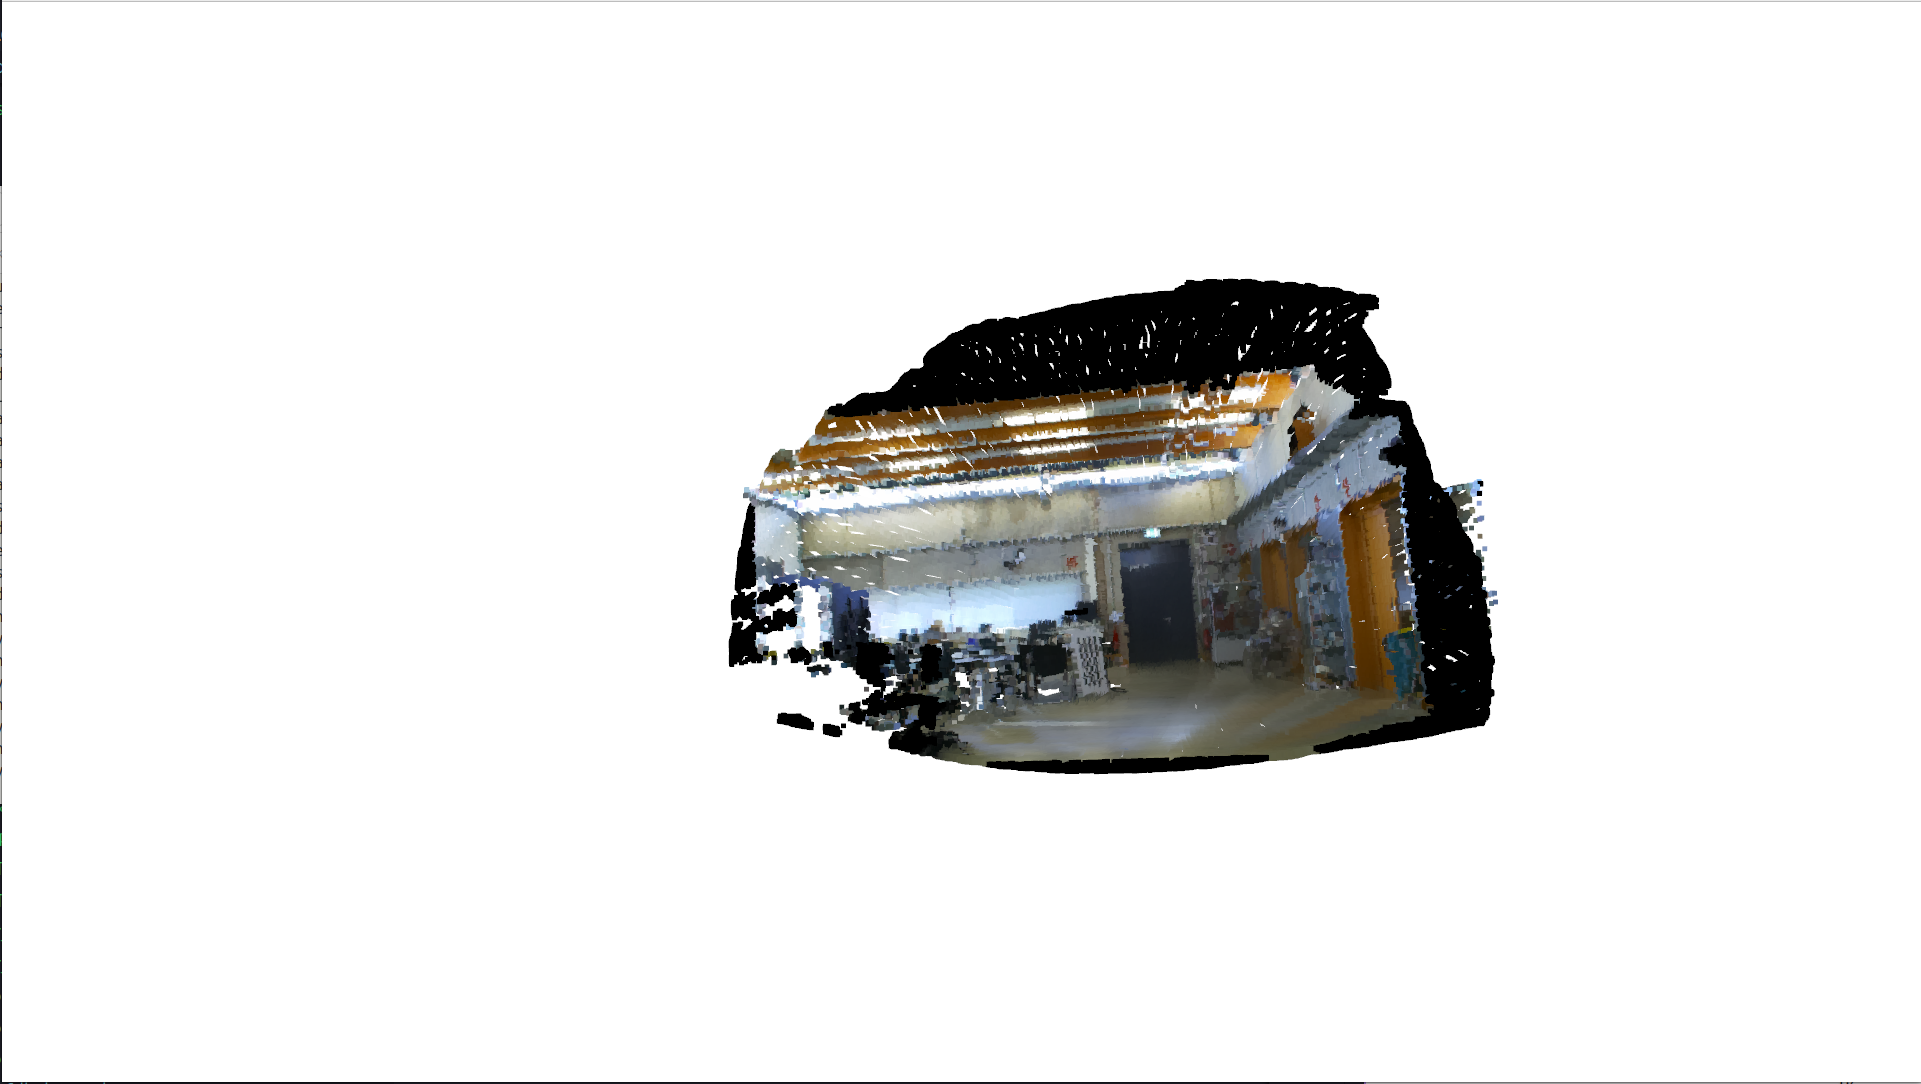
\includegraphics[width=\linewidth]{pics/robo/robo_1/Screenshot from 2025-09-14 18-24-59.png} &
    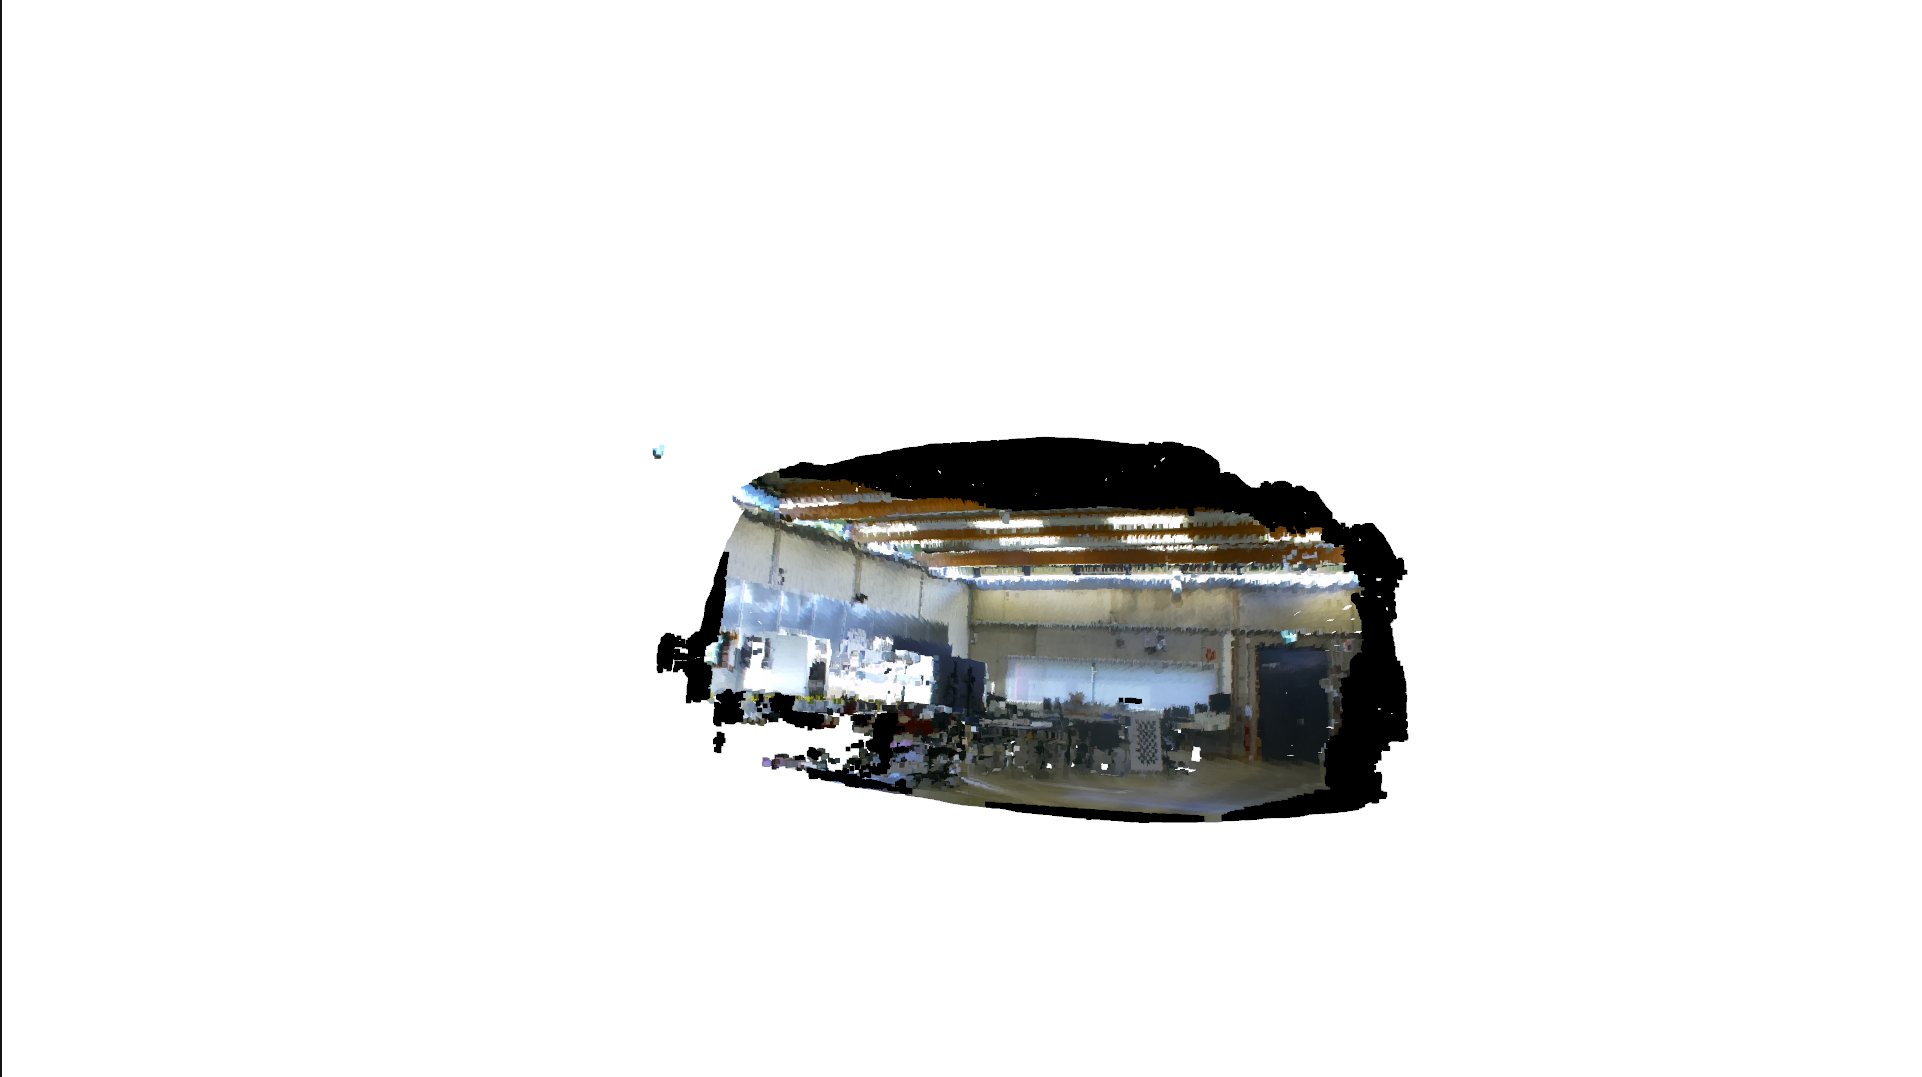
\includegraphics[width=\linewidth]{pics/robo/robo_2/Screenshot from 2025-09-14 18-25-32.png} &
    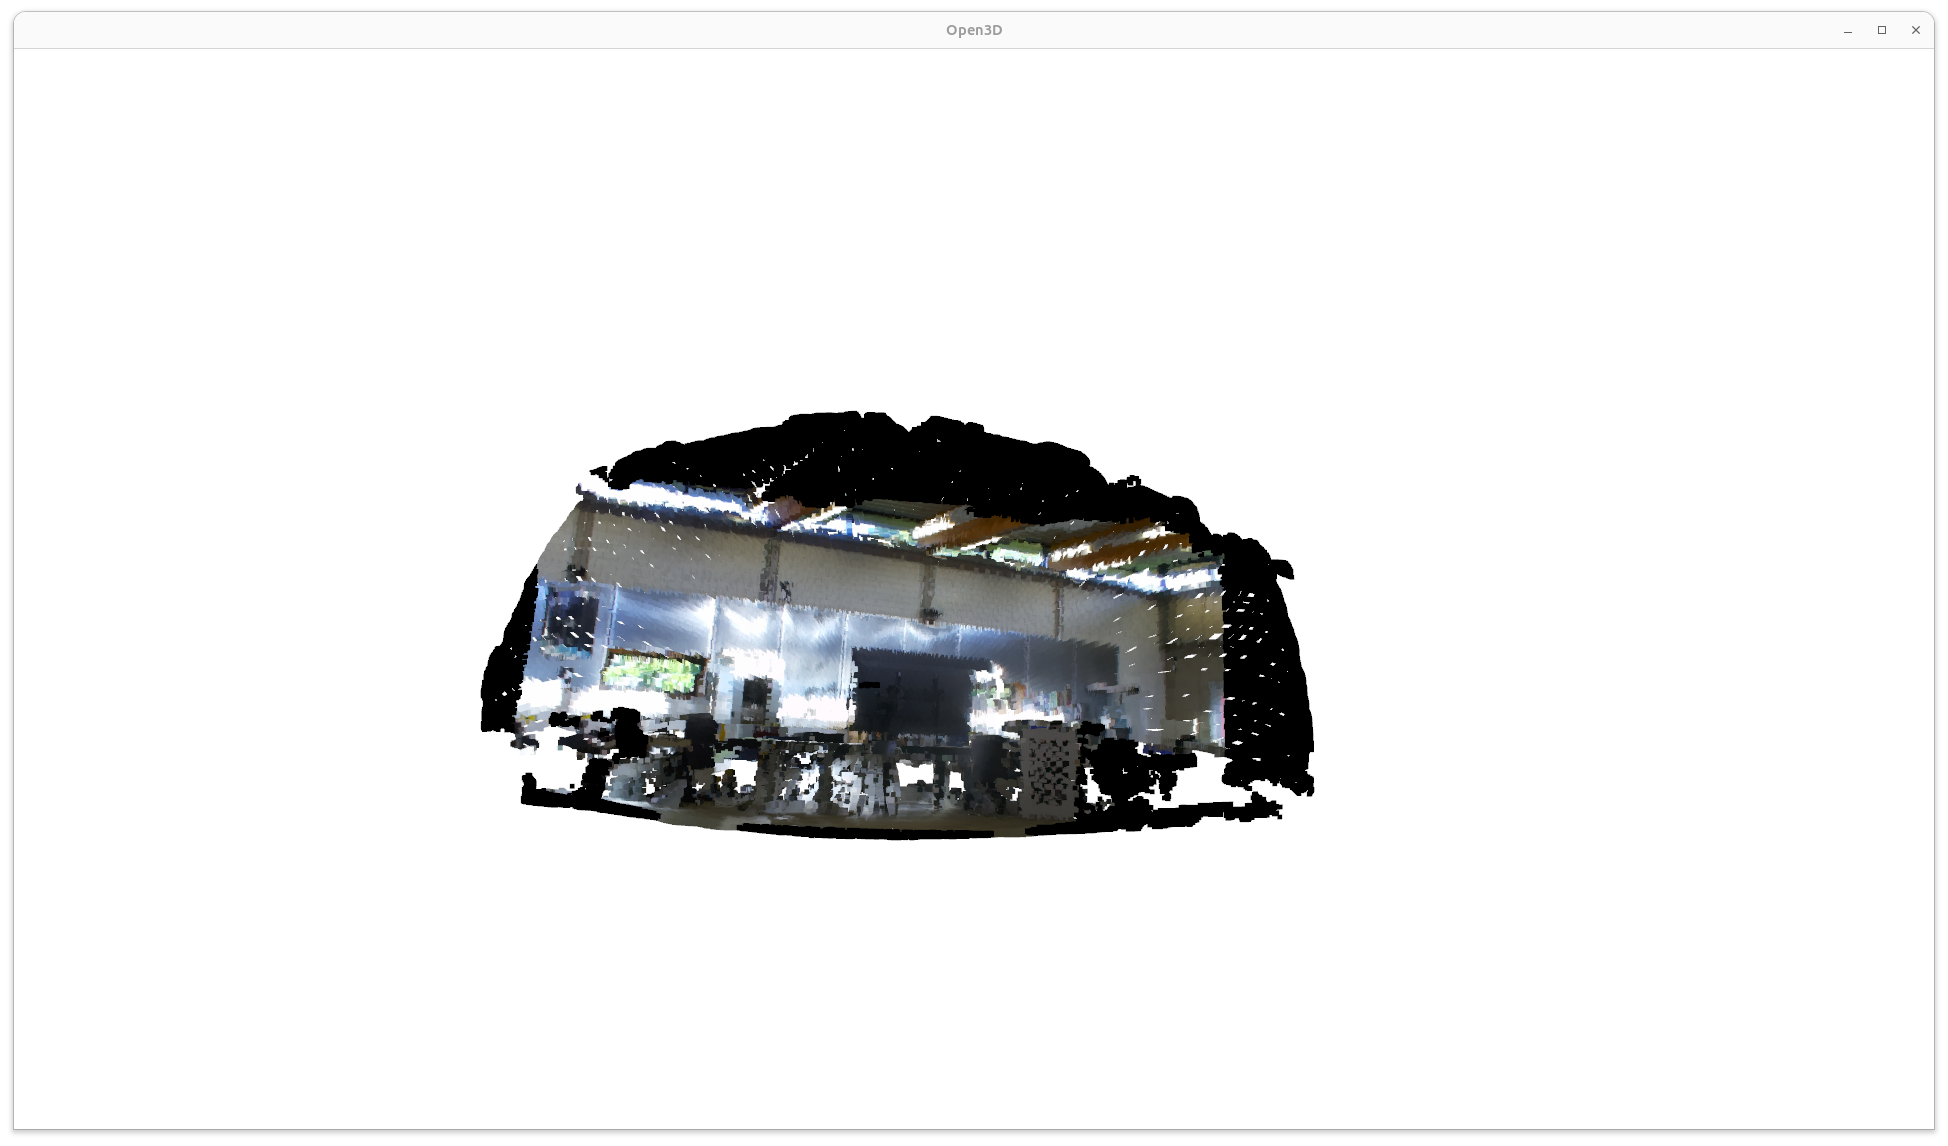
\includegraphics[width=\linewidth]{pics/robo/robo_3/Screenshot from 2025-09-14 18-26-00.png} &
    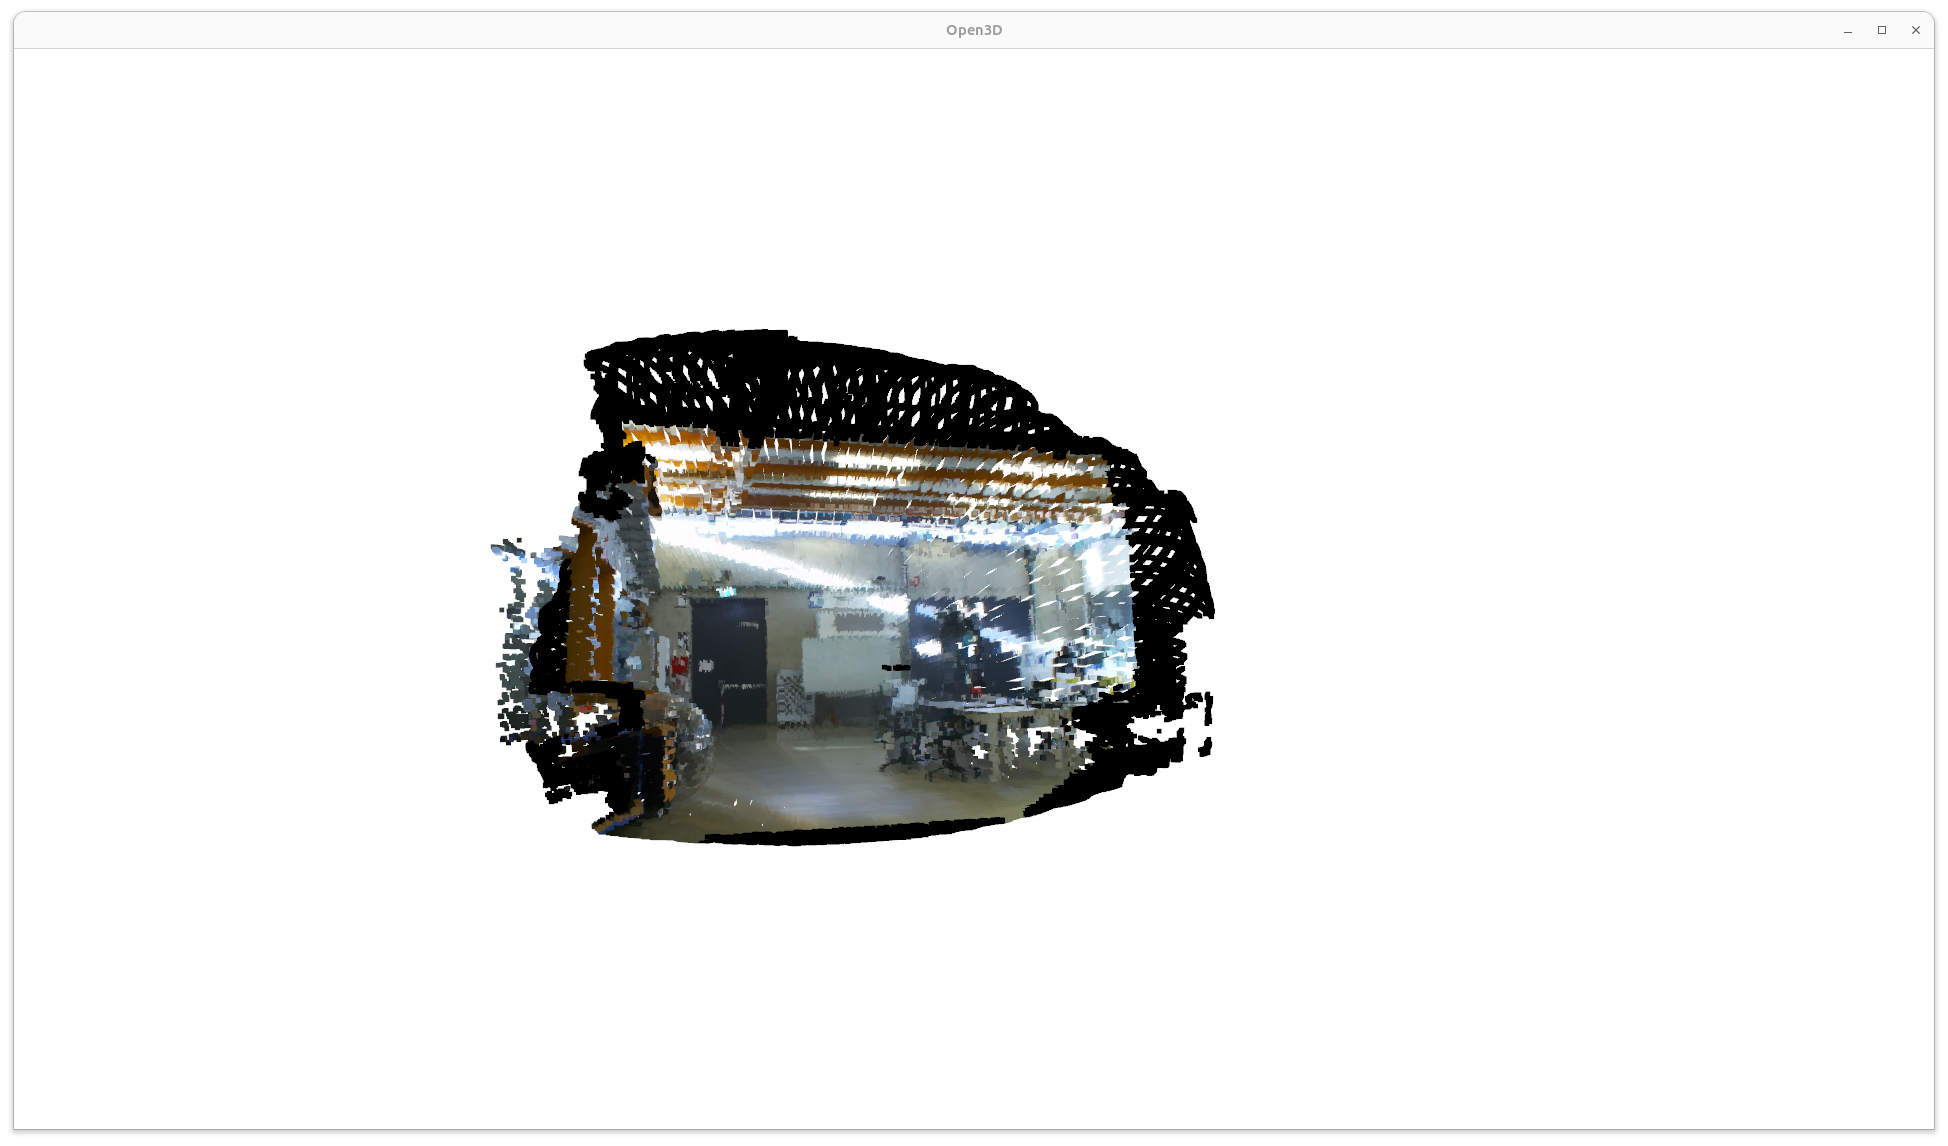
\includegraphics[width=\linewidth]{pics/robo/robo_4/Screenshot from 2025-09-14 18-26-36.png} \\
    \end{tabular}
\end{table}

    \section{Uni--Fusion}

    Unfortunately, the generated RGB-D frames could not be evaluated within the Uni--Fusion framework. The 
    installation of the required software environment on the designated workstation encountered persistent 
    technical issues, which prevented a successful deployment of the pipeline. As a result, the integration 
    and direct testing of the data inside Uni--Fusion was not possible within the scope of this thesis. This 
    limitation should be addressed in future work, as a full evaluation within the intended system would 
    provide a more comprehensive assessment of the quality and usability of the reconstructed depth images.

    %\textcolor{red}{\section{Comparison with Commercial Devices}}

    %In order to assess the performance of the developed handheld device, it is essential to place it in 
    %relation to existing commercial systems. A representative industrial benchmark is the SHARE 
    %S20 LiDAR device \cite{shareS20}, which is offered at a price of approximately 5600~EUR. The S20 
    %provides high accuracy and robustness, making it suitable for professional surveying and industrial 
    %applications. However, the cost of such systems can be prohibitive for many use cases that require 
    %flexibility and affordability, such as rapid prototyping, small-scale cultural heritage projects, 
    %or educational environments. 
%
    %By contrast, the handheld prototype developed in this thesis is based on a low-cost Livox LiDAR 
    %sensor combined with a monocular RGB camera, resulting in a system that can be realized for only a 
    %fraction of the price. While the industrial device achieves superior range and precision, the 
    %prototype demonstrates that competitive results can be obtained with significantly lower hardware 
    %investment. This comparison highlights the potential of low-cost alternatives for practical outdoor 
    %scenarios, where budget limitations often restrict access to high-end equipment. The evaluation thus 
    %underscores the relevance of designing cost-efficient yet reliable RGB-D fusion systems, which can 
    %expand accessibility and enable broader adoption in research and industry.
%
%
    %Table shows that the complete bill of materials amounts to approximately 1{,}327\,€.
    %In other words, the proposed prototype is a genuinely \emph{low-cost} device: compared to an integrated
    %off-the-shelf SLAM sensor such as a SHARE~20 SLAM (ca.\ 5{,}000\,€), the total acquisition cost is
    %about $\approx 3.8\times$ lower, corresponding to a reduction of roughly $\sim 73\%$. Despite the Livox
    %Mid70 being the largest single expense (900\,€), the remainder of the system is built from commodity
    %components (Raspberry~Pi~5 with accessories, low-cost camera module and optics, IMU, and peripherals),
    %which keeps the overall budget modest. This cost profile makes the platform attractive for student projects
    %or small research labs. All prices are approximate and
    %reflect typical market variability at the time of purchase.

\chapter{Conclusion and future work}

The developed handheld scanning system, which is based on a Raspberry Pi~5 in combination with the 
Livox Mid--70 LiDAR sensor, has been successfully implemented and evaluated in the course of this work. 
The data acquisition using the integrated touchscreen operates reliably and provides 
a way of starting and managing the recording process. Furthermore, the subsequent data organization and storage 
follows the structured scheme described in section~\ref{sec:approach}, which ensures that the different 
sensor modalities are consistently aligned in a reproducible file hierarchy. This facilitates both later 
processing and the integration into external frameworks. Nevertheless, several limitations became evident 
during the experiments. One of the most critical aspects is the calibration between the LiDAR sensor and 
the RGB cameras. Inaccuracies in this calibration were clearly observable, for example in the colored 
point clouds (see section \ref{sec:experiments}), where misalignments led to visible distortions and incorrect color assignments. Such errors 
directly affect the quality of the generated data and limit the usability of the results in downstream tasks. 
Another important limitation is related to the inertial measurement unit (IMU). 
Because the Livox Mid--70 has no internal IMU, the external IMU has to get calibrated, which 
was not completed at the time of submission. The imu data is still stored in the output files.
This represents a significant disadvantage, since an accurate 
IMU calibration would considerably improve the performance of scan alignment methods such as Iterative 
Closest Point (ICP) or alternative calibration and registration algorithms. The absence of a factory-calibrated 
IMU is one of the major drawbacks of the Livox hardware, as it complicates the development of a fully 
integrated and robust handheld mapping solution. Despite these shortcomings, the developed software 
pipeline is able to process the recorded data and generate both RGB and depth images.
It remains to be demonstrated whether depth images obtained via interpolation are sufficient for Uni--Fusion.
Should this not hold -- which is plausible when aiming for highly detailed and geometrically faithful reconstructions --
future work ought to consider alternative strategies, such as \emph{ScaleCov} (see section~\ref{sec:sparsedepth}).

The outputs are structured in a way that is compatible with the Uni--Fusion framework.
Although the actual integration and testing within Uni--Fusion could 
not be completed due to technical issues with the target system, the produced results demonstrate that the 
pipeline provides a working foundation.

In summary, despite limited hardware resources and the inherent constraints of the Livox Mid-70, this thesis
demonstrates that a functional, portable and cost-efficient handheld RGB-D scanner can be built around a
Raspberry Pi 5. We designed and assembled the device, integrated a monocular camera with the LiDAR and
established calibration and synchronization procedures, alongside a processing pipeline that produces
depth images and RGB-D outputs suitable for downstream frameworks such as Uni--Fusion. While the present
accuracy is not yet sufficient for high-precision applications, the collected data already provide a sound
basis for further processing and integration. The only objective not completed within the thesis timeframe
was the end-to-end evaluation in Uni--Fusion; future work should finalize the IMU calibration and conduct
a full Uni--Fusion evaluation and benchmarking on
representative datasets. Addressing these points will increase accuracy and reliability and broaden the
system's applicability to practical 3D mapping and multimodal reconstruction scenarios.


\newpage

\appendix
\chapter{Drawings handheld Device}
\label{app:handheld_drawings}
\includepdf[pages=-]{pics/Device Images/Main_Device_Ansichten.pdf}
\includepdf{pics/Device Images/H99_Halterung_Drawing v2.pdf}


% DON'T set \bibliographystyle here -- use the documentclass option instead
\bibliography{papers}
% Make sure all citation keys used in \cite{...} exist in papers.bib

\closing %%%%%%%%%%%%%%%%%%%%%%%%%%%%%%

\end{document}
